\section{1M1 Messung der Erdbeschleunigung mit dem Pendel}

\begin{aufgabe}{Grundlagen}
  Knappe Beschreibung der theoretischen Grundlagen, Angabe der
  benötigten Formel(n), ohne Herleitung. Definition der verwendeten
  Formelzeichen.
\end{aufgabe}

% Bitte belassen Sie die Aufgabentexte in Ihrem Protokoll und beginnen
% Sie hier mit der Lösung der ersten Aufgabe:
Im Versuch wird die Erdbeschleunigung mit einem Pendel experimentell bestimmt.\\
Die theoretische Grundlage dazu ist das mathematische Pendel. Hier wird die Annahme eines masselosen Fadens sowie einer punktförmigen, schweren Masse getroffen. Die Schwerkraft auf die Pendelmasse lautet:\\
\[
F_g = m_S \cdot g 
\]
Wenn das Pendel aus der Ruhelage ausgelenkt wird, wirkt eine ein rückstellendes Drehmoment. Dieses ergibt sich aus:
\[
D_R = F_R \cdot l = F_g \cdot sin(\varphi) \cdot l
\]
wobei $l$ die Länge des Fadens und $\varphi$ den Auslenkwinkel zwischen Ruhelage und Faden beschreibt. Mit der Kleinwinkelnäherung $sin(\varphi) \approx \varphi$, welche für $\varphi<5^{\circ}$ noch erfüllt ist,  folgt die Bewegungsgleichung: \\
\[
J \cdot \ddot{\varphi} = -F_g \cdot sin(\varphi) \cdot l \approx -m_S \cdot g \cdot \varphi \cdot l  \]
wobei $J = m_T \cdot l^2$ das Trägheitsmoment der Pendelmasse nach dem Steiner'schen Satz beschreibt und $m_T$ die träge Masse des Pendelkörpers ist. Da die träge der schweren Masse gleicht, folgt:
\[
\ddot{\varphi} = - \frac{g}{l} \cdot \varphi
\] 
Dies ist eine lineare, homogene Differentialgleichung zweiter Ordnung. Die Lösung ergibt sich aus einer harmonischen Oszillation: 
\[
\varphi(t) = \varphi_{max} \cdot cos(\omega_{mat} t)
\]
mit $\omega_{mat} = \sqrt{\frac{g}{l}}$.
Als Schwingungsdauer für das Pendel ergibt sich:
\[
T = \frac{2\pi}{\omega_{mat}} = 2\pi \cdot \frac{l}{g}
\]
Im Versuchsaufbau handelt es sich jedoch um ein physikalisches Pendel. Hierbei wird die Näherung eines masselosen Fadens und einer Punktmasse aufgelöst. Die Fadenlänge bzw. Stangenlänge $l$ bezieht sich dann auf den gemeinsamen Schwerpunkt der Pendelstange und -körper. $J$ beschreibt dann das Gesamtträgheitsmoment des Systems, welches eine komplexe Form aufgrund der Pendelstange aufweist. Formal ergibt sich für die Bewegungsgleichung mit der Kleinwinkelnäherung:
\[
J_{ges} \cdot \ddot{\varphi} = -m_{ges } \cdot g \cdot \varphi \cdot l_{S} 
\]
Wie zuvor ist die Lösung dieser Differential-Gleichung eine harmonische Oszillation. Die Kreisfrequenz ergibt sich demnach zu:
\[
\omega^2 = \frac{m\cdot g\cdot l_s}{J_{ges}}
\]
und somit
\[
T^2 = \frac{4\pi^2}{g}\cdot \frac{J_{ges}}{m_{ges}l_s}
\]
Um die komplexe Berechnung des gemeinsamen Schwerpunktes vom Winkelaufnehmer-Profil, Stange und Pendelkörper, siehe Abbildung \ref{fig:aufbau_pendel}, zu umgehen, wird die Schwingung des Pendels mit und ohne Pendelkörper betrachtet. Zunächst wird die Schwingfrequenz ohne Pendelkörper ($\omega_{st}$) bestimmt. Anschließend wird der Pendelkörper angebracht und $l_s$ variiert, bis für die Schwingfrequenz $\omega = \omega_{st}$ gilt. Mit
\[
\omega_{st}^2 = \frac{D_{st}}{J_{st}} \quad \quad \omega_{p}^2 = \frac{D_{p}}{J_{p}}
\]
und
\[
\omega^2 = \frac{D_{st}+D_p}{J_{st}+J_p} = \omega_{p}^2 \cdot \frac{1+\frac{D_{st}}{D_p}}{1+\frac{J_{st}}{J_p}} = \omega_{st}^2 \cdot \frac{1+\frac{D_p}{D_{st}}}{1+\frac{J_p}{J_{st}}}
\]
folgt mit $\omega = \omega_{st}$
\[
\frac{J_p}{J_{st}} = \frac{D_p}{D_{st}} \Leftrightarrow \frac{D_p}{J_p} = \frac{D_{st}}{J_{st}} \Leftrightarrow \omega_{p}^2 = \omega_{st}^2
\]
und somit
\[
\omega_{p}^2 = \omega^2.
\]
Wenn also die Schwingfrequenz $\omega$ des gesamten Pendels mit der Schwingfrequenz $\omega_{st}$ synchronisiert wird, kann die Masse der Stange aus der Betrachtung ausgelassen werden. Es muss lediglich die Schwingung des ausgedehnten Pendelkörpers betrachtet werden. Da dieser die Geometrie eines Zylinders mit Radius $r_p$ aufweist welcher um $l_p$ von der Rotationsachse verschoben ist, ergibt sich unter Beachtung der Rotationsachse und des Steiner'schen Satzes das Trägheitsmoment zu:
\[
J_p = \frac{1}{2} m_p r_p + m_p l_p^2
\]
Für die Kreisfrequenz folgt:
\[
\omega^2 = \frac{D_p}{J_p} = \frac{m_p\cdot g \cdot l}{\frac{1}{2} m_p r_p + m_p l_p^2}
\]
Für $g$ ergibt sich
\begin{equation}
g = \omega^2 l_p \Bigg(1+\frac{r_p^2}{2\cdot l_p^2}\Bigg) = \frac{4 \pi^2}{T^2} l_p \Bigg(1+\frac{r_p^2}{2\cdot l_p^2}\Bigg).
\end{equation}


 
\begin{aufgabe}{Versuchsaufbau und Versuchsdurchführung}
	Beschreibung des Versuchsaufbaus einschließlich beschrifteter Skizze
	oder Foto. Beschreibung der Versuchsdurchführung: Handgriffe an der
	Apparatur, verwendete Messwerterfassungseinstellungen, Messbereiche,
	Triggerbedingungen, etc.
\end{aufgabe}

\textbf{Zum Aufbau:} \\

Für den Versuch wird zunächst ein stabiles Dreibein benötigt. Dieses besteht aus drei Metall-Stangen, welches wir vertikal an einem Tisch mit Tischklemmen eingespannt haben. An diesen drei Stangen haben wir wiederum drei Metall-Stangen mit Verbindungsmuffen horizontal eingespannt, sodass von oben betrachtet ein Dreieck entstand. Der Aufbau des Dreibeins ist in Abbildung \ref{fig:Aufbau_Dreibein} ersichtlich. Dabei haben wir mit einer Wasserwaage überprüft, ob die horizontale Stange an der die Pendel angebracht werden, tatsächlich waagerecht ist. Dieser Prozess ist in Abbildung \ref{fig:tarierung_dreibein} dargestellt. An dieser Stange haben wir dann zwei Winkelaufnehmer mit Verbindungsmuffen befestigt. Auch dabei haben wir auf eine waagerechte Ausrichtung geachtet. Im Winkelaufnehmer ist eine Hall-Sonde verbaut, um die magnetische Feldstärke orthogonal zur Ausrichtung des Pendels in Ruhelage zu messen. Dieses wird in eine Hall-Spannung translatiert, welche proportional zum Sinus des Auslenkwinkels bzw. für $\varphi<5^\circ$ proportional zum Auslenkwinkel ist. Die Winkelaufnehmer werden von jeweils einem Kabel mit einer Spannung versorgt. Über ein weiteres, zweiadriges Kabel haben wir die Winkelaufnehmer mit dem Sensor-Cassy verbunden, um die ausgegebene Spannung messen zu können. Dabei ist der in Abbildung \ref{fig:Aufbau_Dreibein} links zu sehende Winkelaufnehmer mit dem Eingang A des Sensor-Cassys verbunden und der rechts zu sehende mit Eingang B. Der Sensor-Cassy ist mit dem Laptop verbunden. Der Aufbau des Dreibeins mitsamt der Winkelaufnehmer ist in Abbildung \ref{fig:Aufbau_Dreibein} dargestellt. Die Verkabelung ist in Abbildung \ref{fig:verkabelung} dargestellt. 

\begin{figure}[H]
	\centering
	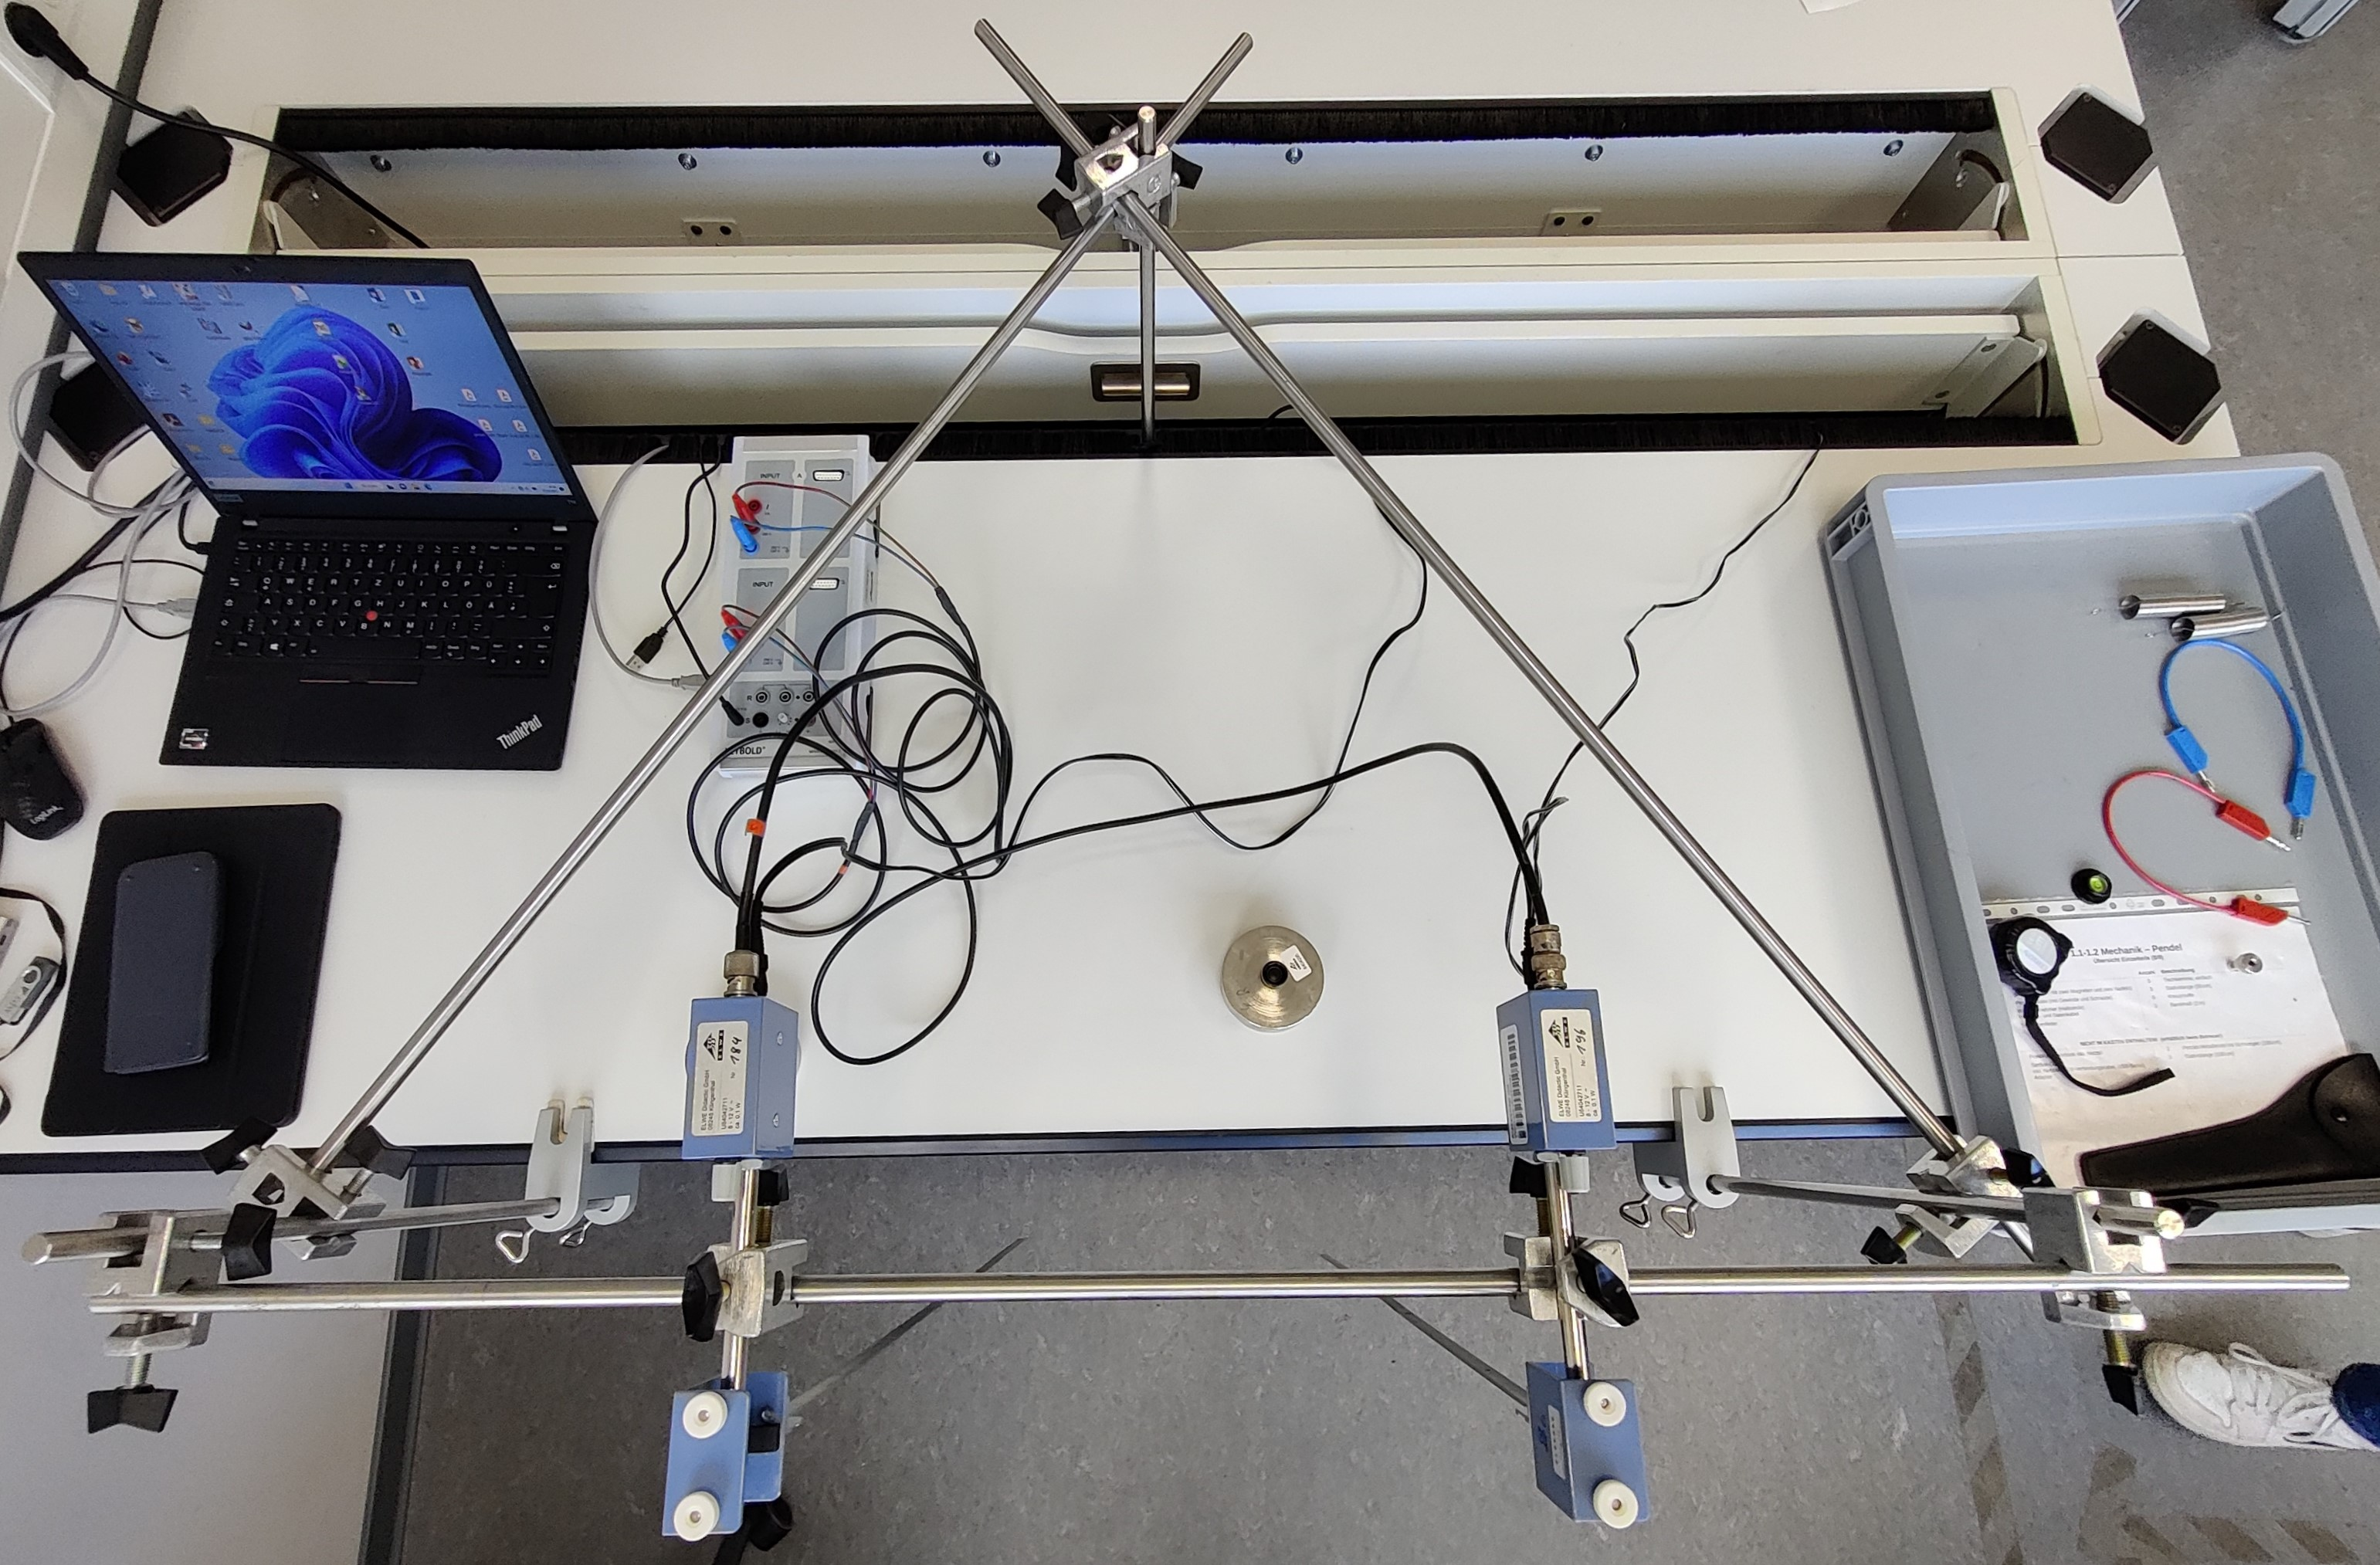
\includegraphics[width=1\textwidth]{Aufbau_Dreibein.jpg}
	\caption{Aufbau des Dreibeins im Labor}
	\label{fig:Aufbau_Dreibein}
\end{figure}
\begin{figure}[H]
	\centering
	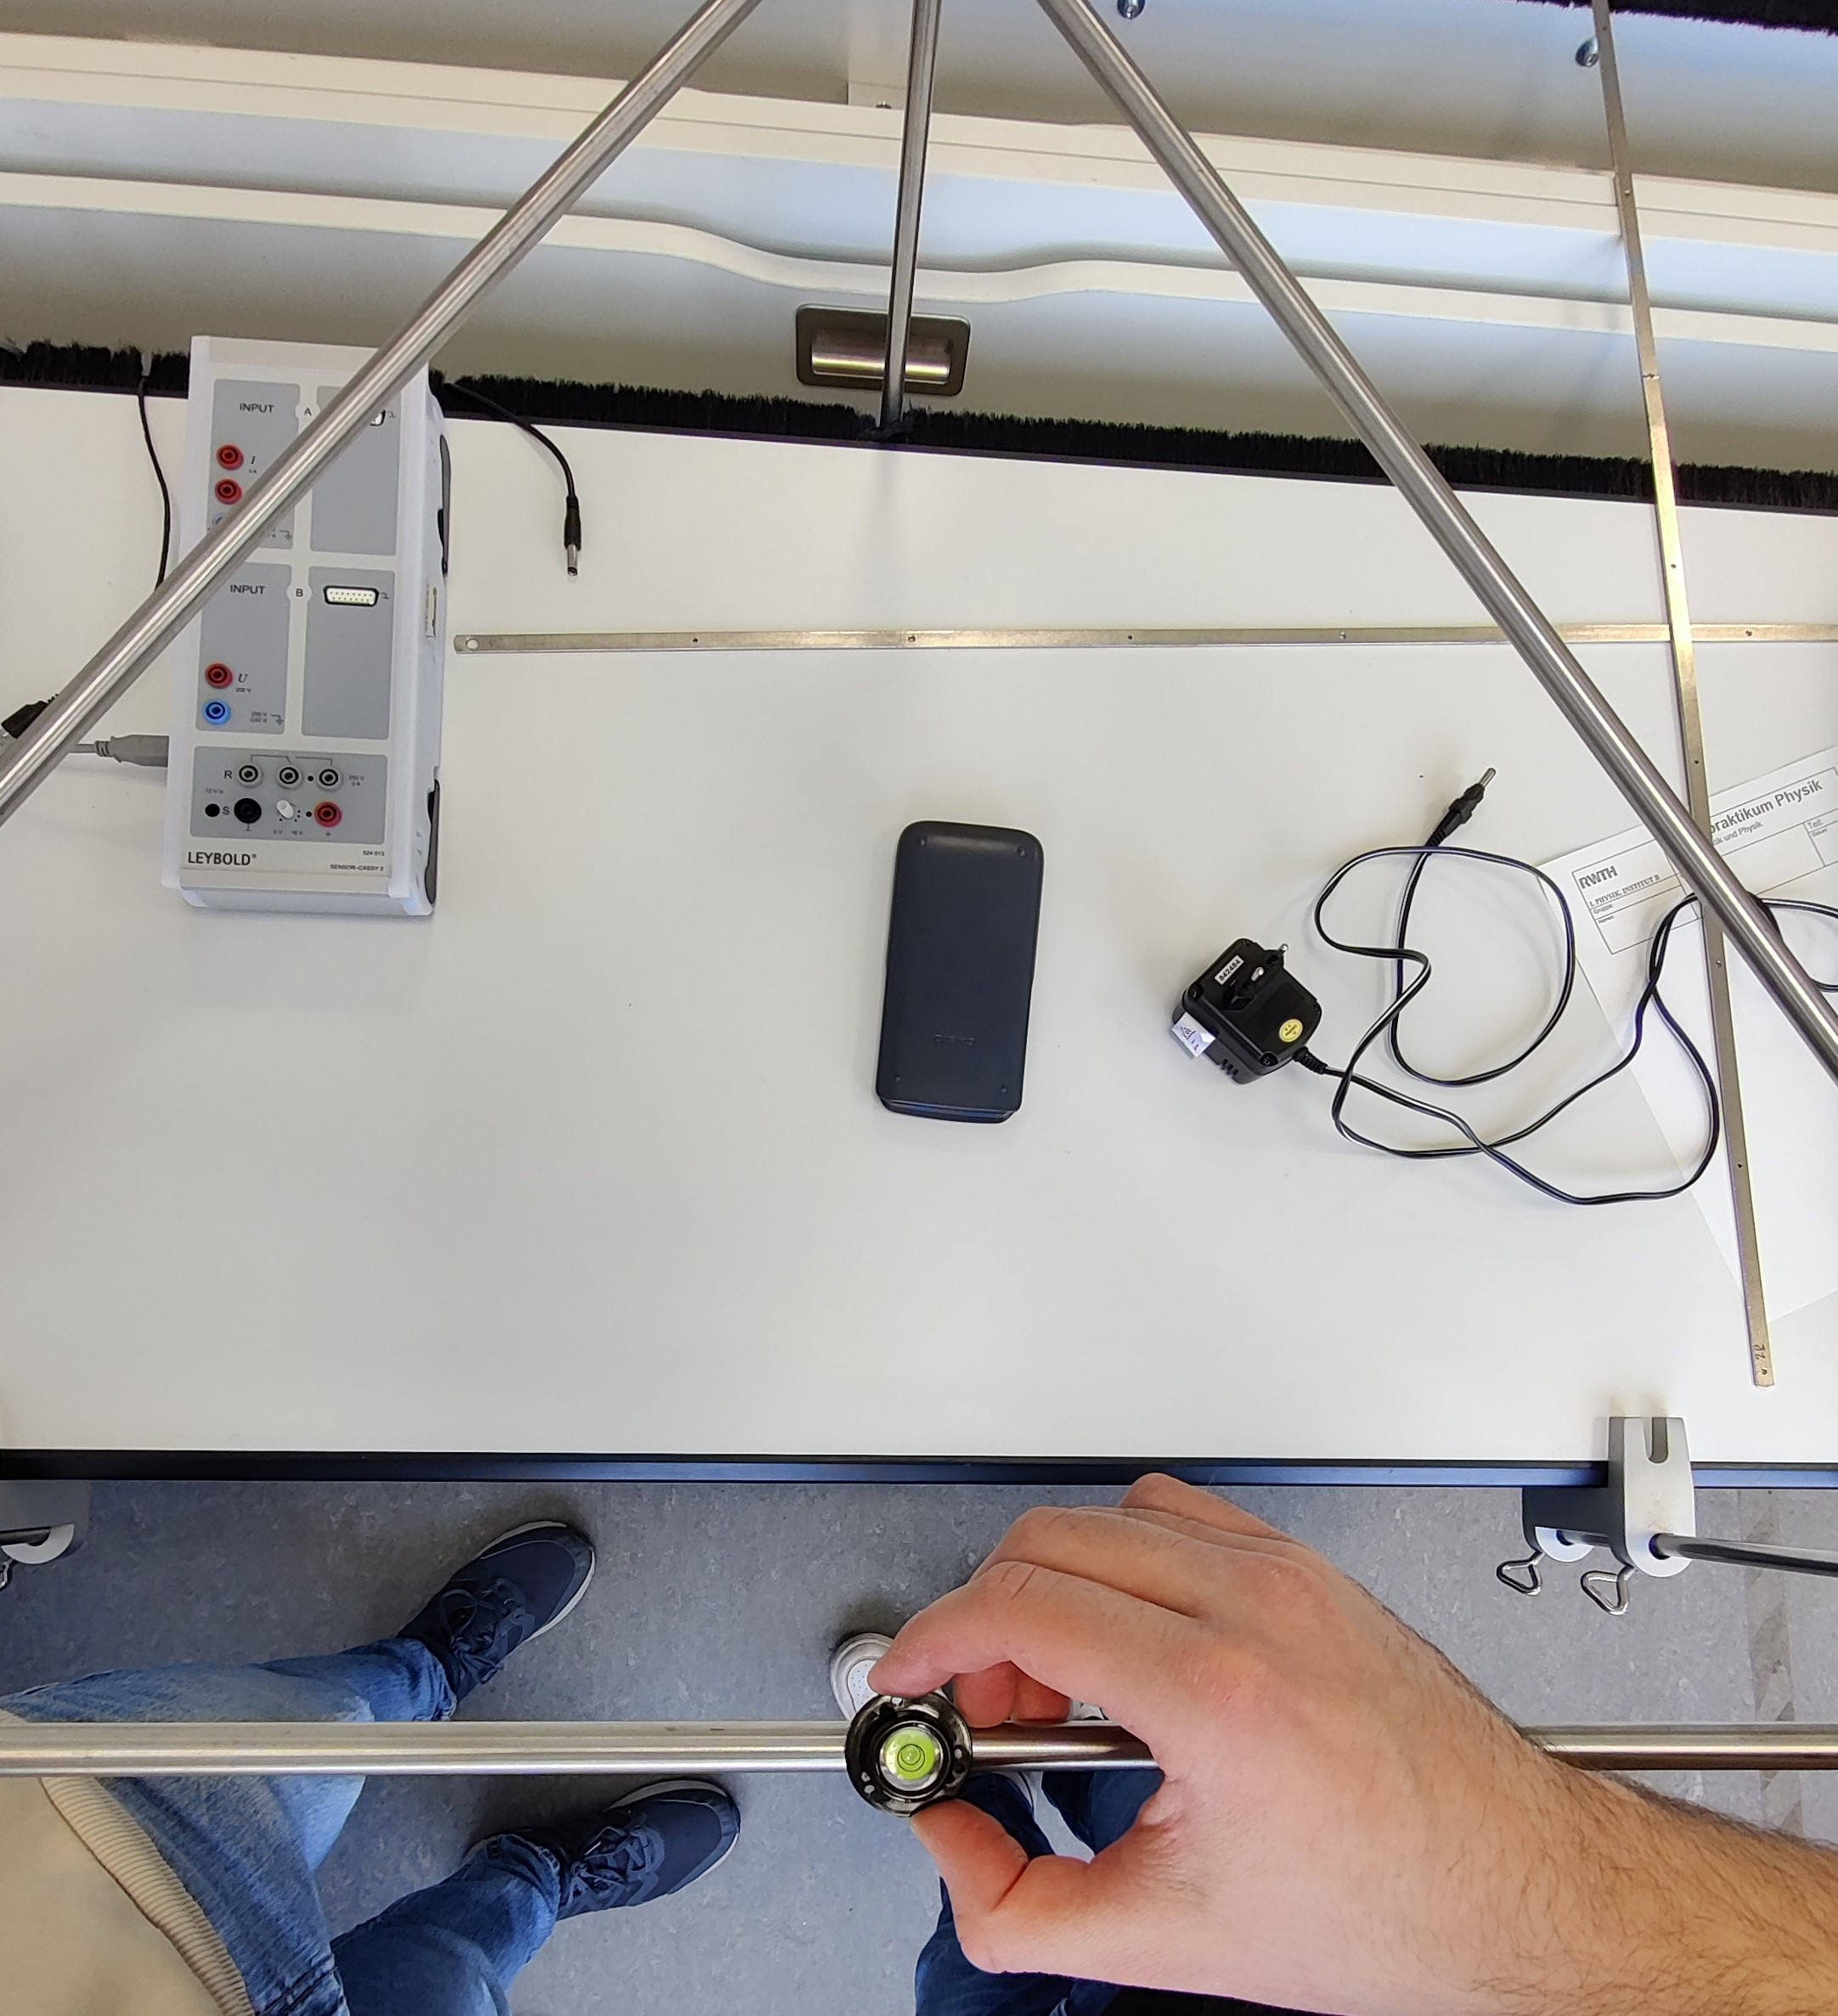
\includegraphics[width=1\textwidth]{tarierung_dreibein.jpg}
	\caption{Prüfung der Neigung des Dreibeins}
	\label{fig:tarierung_dreibein}
\end{figure}
\begin{figure}[H]
	\centering
	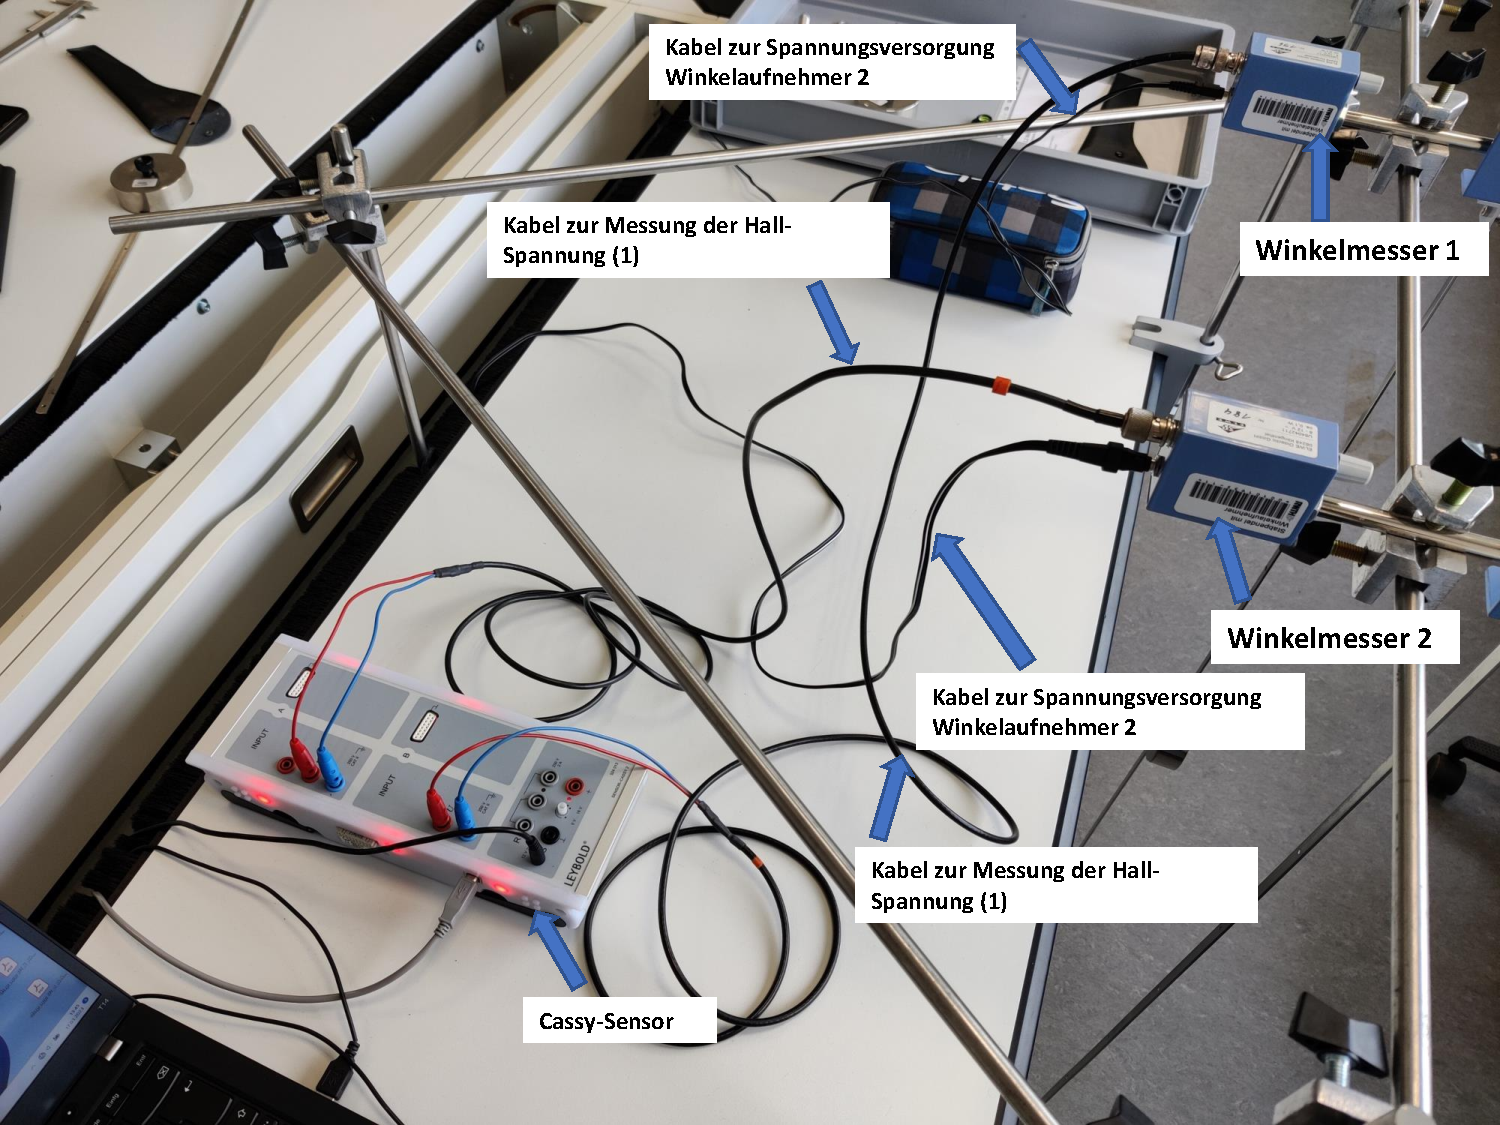
\includegraphics[width=1\textwidth]{verkabelung.pdf}
	\caption{Verkabelung der Winkelaufnehmer}
	\label{fig:verkabelung}
\end{figure}

Das Pendel besteht aus drei Elementen. Das Winkelaufnehmerprofil ist C-förmig und weist zwei dünne Spitzen auf, welche in einer Kerbe des Winkelaufnehmers aufliegen. In der Innenseite des Winkelaufnehmerprofils ist oben und unten jeweils ein Permanentmagnet angebracht. An dem Profil ist die eigentliche Pendelstange angebracht. An dieser wird der zylindrische Pendelkörper angeschraubt. Die Länge a beschreibt die Distanz von dem Ende der Spitze bis zur Innenseite des Winkelaufnehmerprofils. Die Länge b beschreibt die Distanz von der unteren Innenseite des Winkelaufnehmerprofils bis zum Rand des Pendelkörpers. D beschreibt den Durchmesser des zylindrischen Pendelkörpers. $l_p$ beschreibt die resultierende Pendellänge. Diese definiert als die Distanz vom Pivot-Point bis zum Schwerpunkt der Pendelmasse. Es gilt:
\[l_p = a +b+ \frac{D}{2}\]
Ein schematischer Aufbau des gesamten Pendels ist in Abbildung \ref{fig:aufbau_pendel} dargestellt. \\
\begin{figure}[H]
	\centering
	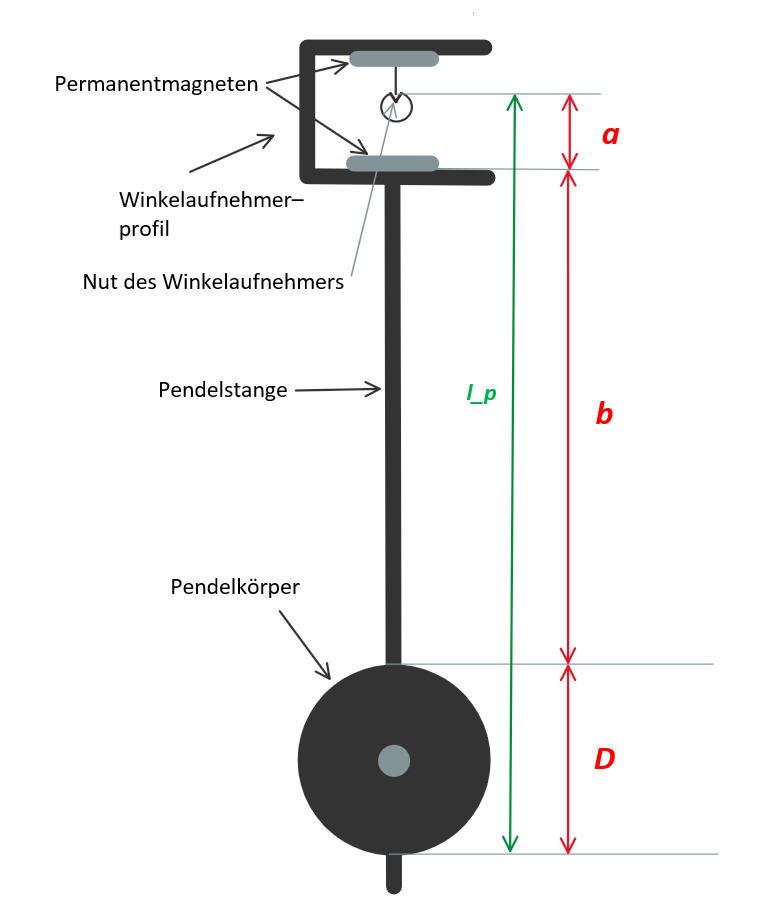
\includegraphics[width=1\textwidth]{aufbau_pendel.png}
	\caption{Schematischer Aufbau des Pendels}
	\label{fig:aufbau_pendel}
\end{figure}
Das gesamte Pendel wird dann mit den Spitzen in die Nut des Winkelaufnehmers gehängt. Wenn das Pendel schwingt, dann rotieren die Spitzen innerhalb der Nut. Der Winkelaufnehmer rotiert nicht. Eine Nahaufnahme ist in Abbildung \ref{fig:nahaufnahme_pivotpoint} ersichtlich.
Insgesamt werden zwei Pendel an der Stange nach diesem Aufbau montiert. Das in Abbildung \ref{fig:aufbau_pendel1_pendel2} links dargestellte Pendel wird im folgenden als Pendel 2 bezeichnet. Das rechts dargestellte als Pendel 1.  \\
\begin{figure}[H]
	\centering
	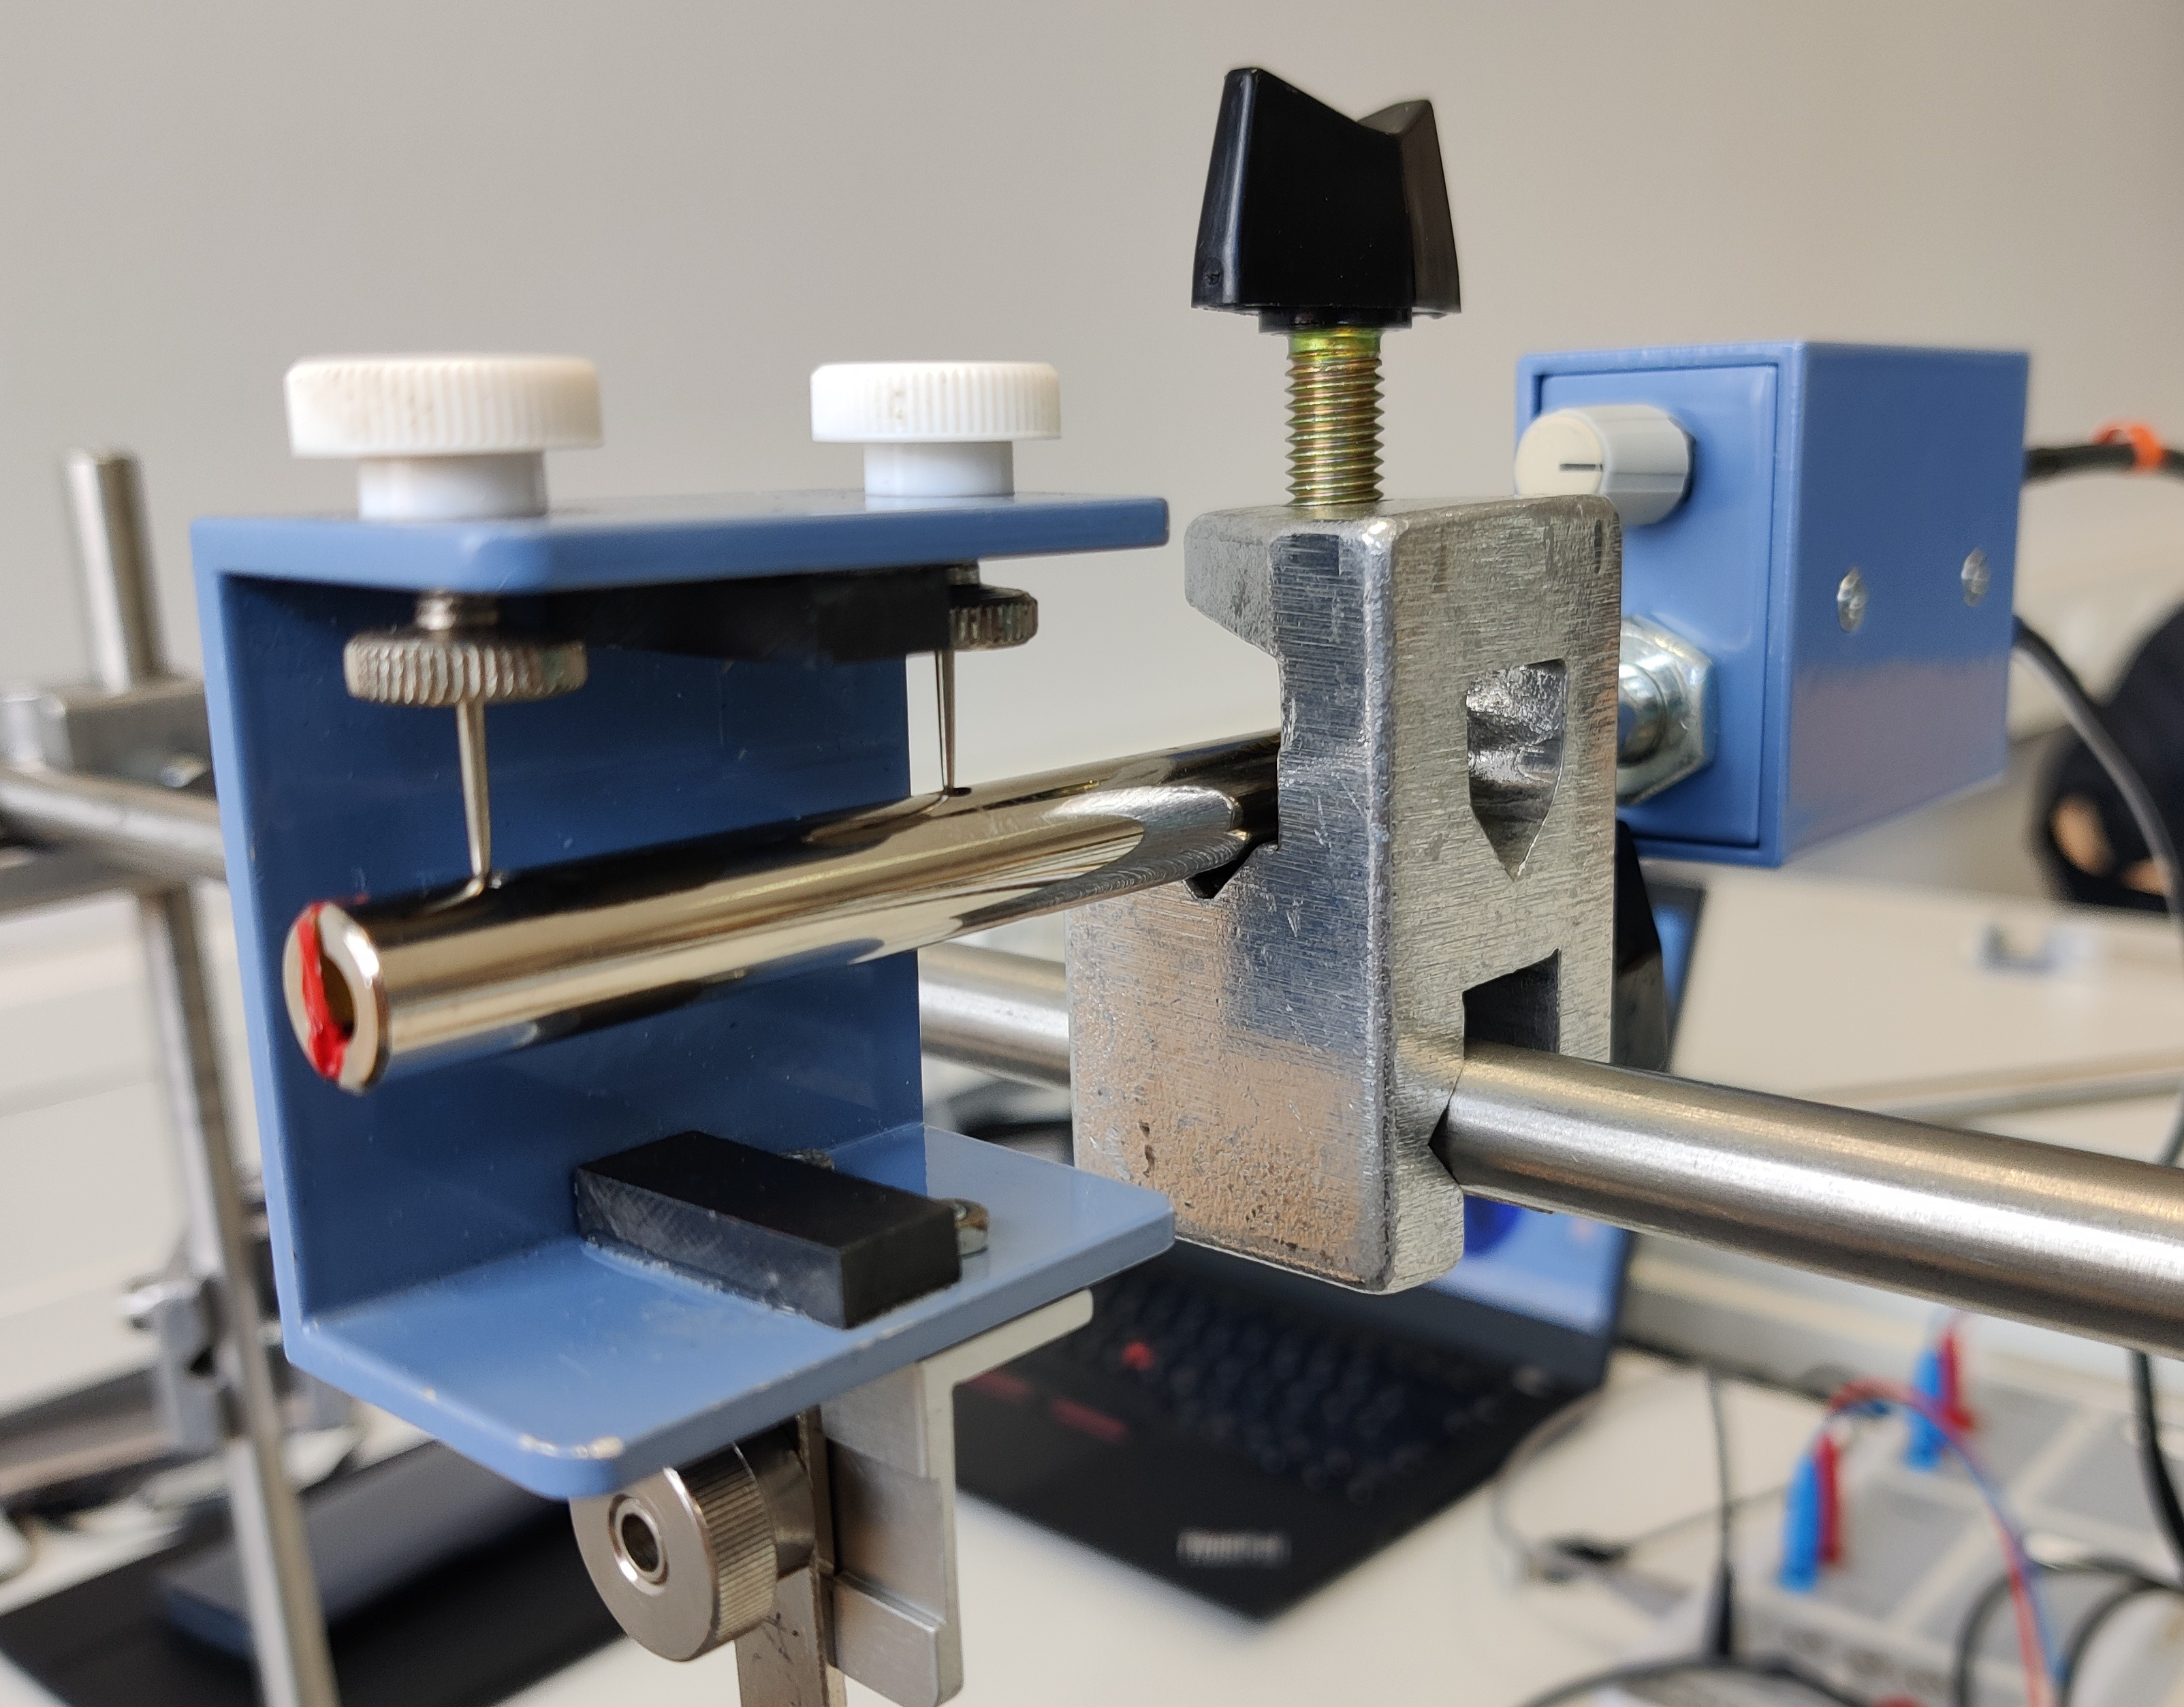
\includegraphics[width=1\textwidth]{nahaufnahme_pivotpoint.jpg}
	\caption{Nahaufnahme des Pivot-Points}
	\label{fig:nahaufnahme_pivotpoint}
\end{figure}
\begin{figure}[H]
	\centering
	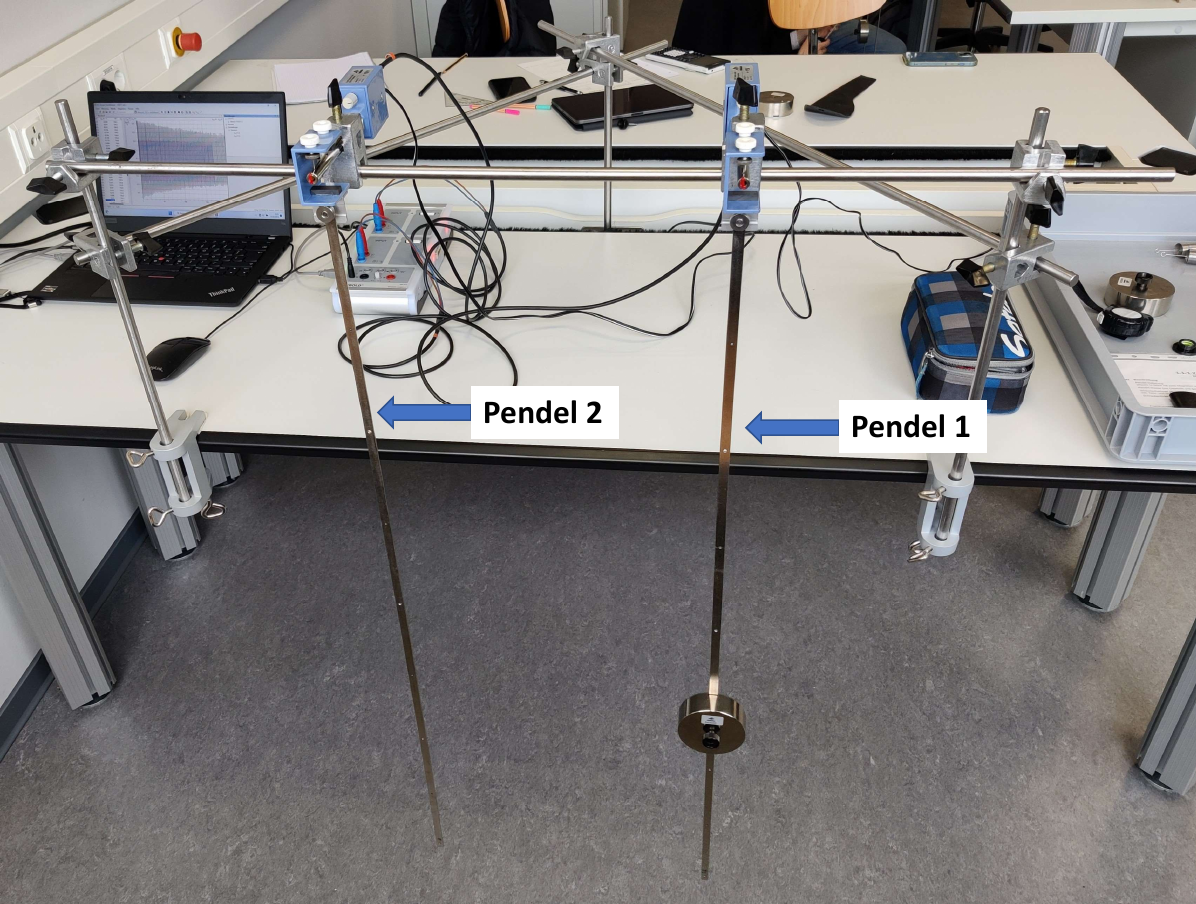
\includegraphics[width=1\textwidth]{aufbau_pendel1_pendel2.png}
	\caption{Aufbau der beiden Pendel 1 und 2}
	\label{fig:aufbau_pendel1_pendel2}
\end{figure}

\textbf{Zur Durchführung:}\\
Bevor wir mit dem Versuch begonnen haben, haben wir zunächst Markierungen gesetzt, um das Pendel nicht weiter als $\varphi=5 ^\circ$ auszulenken. Dazu haben wir grob den Abstand $h \approx 117cm$ vom Pivot-Point bis zum Boden gemessen. Nach der Kleinwinkelnäherung gilt $tan(\varphi) \approx \varphi = \frac{x}{h}$ wobei $x$ die \textcolor{red}{Projektion der Auslenkung auf den Boden beschreibt}. Für $\varphi < 5^\circ$ erhalten wir für die maximale Auslenkung circa $h<10cm$. Wir haben anschließend Markierungen auf dem Boden gesetzt, welche im Abstand von circa $x=9cm$ im Bezug zur jeweiligen Ruhelage der Pendel gesetzt wurden. Dies ist in Abbildung \ref{fig:Markierung_max_Auslenkwinkel} dargestellt. 
\begin{figure}[H]
	\centering
	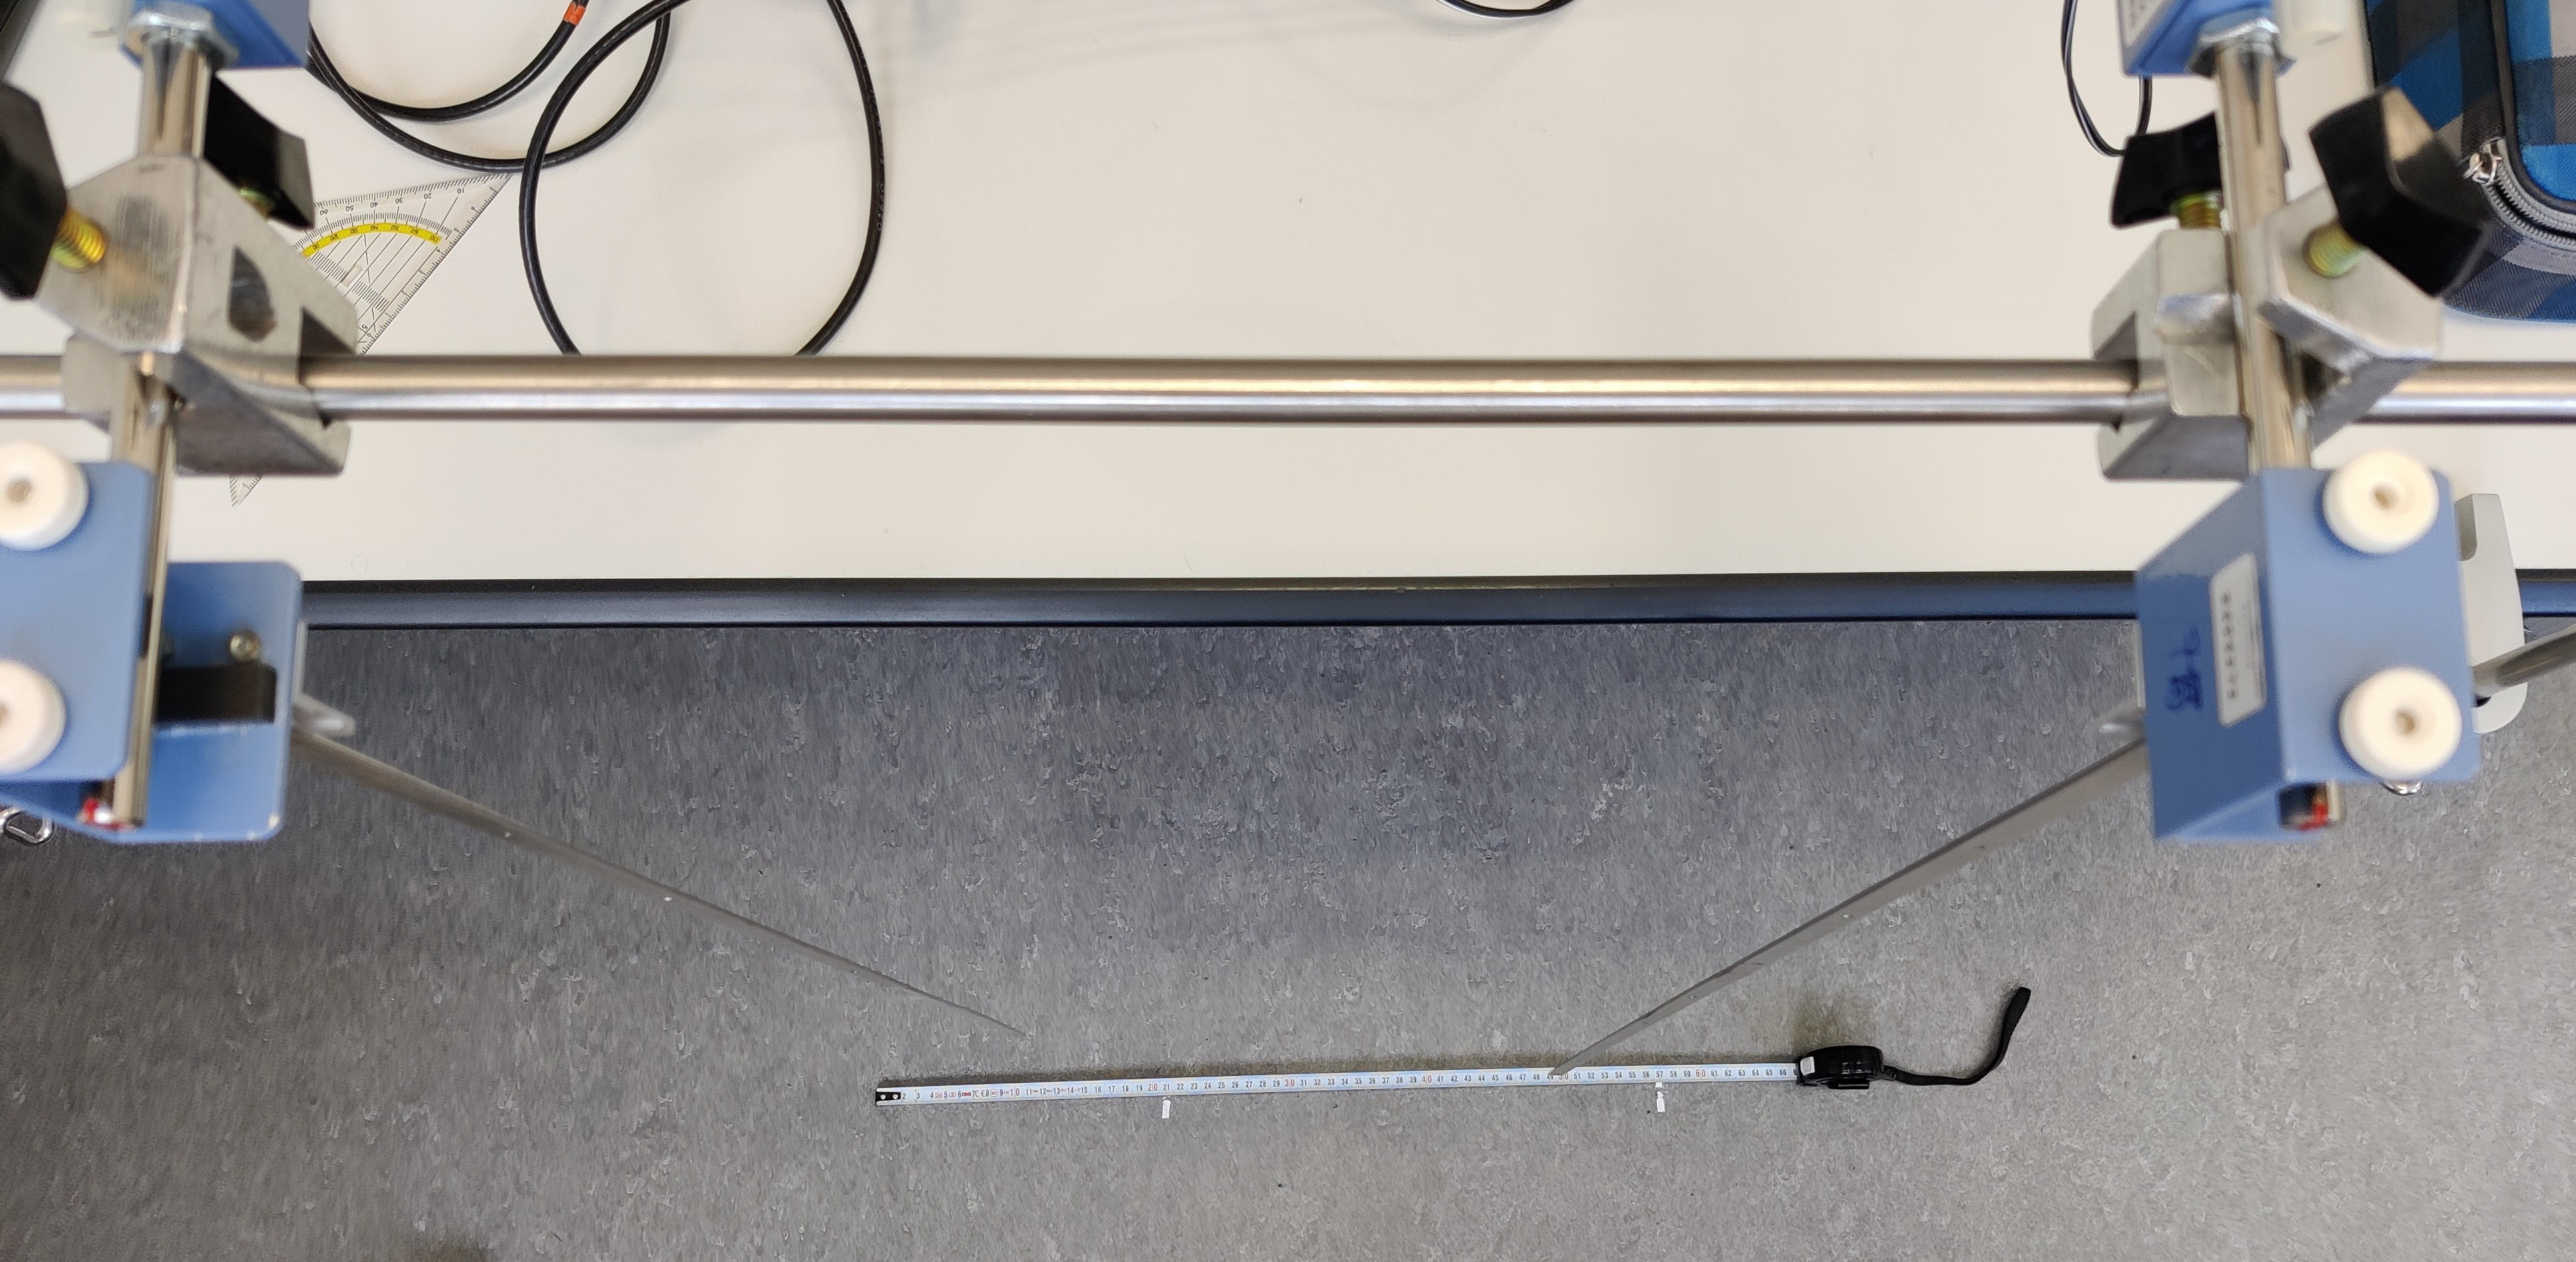
\includegraphics[width=1\textwidth]{Markierung_max_Auslenkwinkel.jpg}
	\caption{Markierungen für den maximalen Auslenkwinkel}
	\label{fig:Markierung_max_Auslenkwinkel}
\end{figure}
Vor der ersten Messreihe haben wir beide Pendel ausgelenkt und schwingen lassen. Optisch haben wir das Pendel bestimmt, welches ruhiger schwingt. Dies war Pendel 1. Mit diesem Pendel haben wir im folgenden alle Messreihen aufgenommen.\\
Wir haben zunächst eine kurze Probemessung mit einer Messzeit von $20s$ und einem Messintervall von $20ms$  für beide Pendel durchgeführt. Über eine schnelle Peak-Analyse in Cassy-Lab haben wir jeweils zwei Peaks bestimmt, welche 10 Perioden auseinander lagen, und das daraus resultierende $\Delta t$ bestimmt bzw. $T$ für Pendel 1 und 2 bestimmt.\\
Mit 
\[T=\frac{t_2-t_1}{10}
\]
und 
\begin{table}[hb]
	\centering
	\caption{Probemessung zur Bestimmung von $T_1$ und $T_2$}
	\label{tab:messwerte_oszi}
	\begin{tabular}{|c|c|c|c|}
		\hline
		Pendel & $t_1$ & $t_2$ \\
		\hline
		$1$ & $1.97s$ & $18.54s$\\
		\hline
		$2$ & $1.97s$ & $18.52s$\\
		\hline
	\end{tabular}
\end{table}\\

ergibt sich $T_1 = 1.657$ und $T_2=1.655s$. Da diese Messung nur zu einer groben Orientierung dient, haben wir auf ein Bestimmen der Unsicherheiten verzichtet. Aus der Probemessung konnten wir schließen, dass beide Pendel in etwa die gleiche Schwingfrequenz aufweisen. Weiterhin konnten wir so die Gesamtmesszeit für die folgenden Messungen bestimmen. Da in etwa 100-120 Perioden aufgezeichnet werden sollen, haben wir uns für eine Gesamtmesszeit von $200s$ entschieden. Das Messintervall haben wir als $20ms$ gewählt. Wir haben in keiner Messung einen Trigger verwendet. Für die Spannungsmessung haben wir einen Messbereich von $\pm 1V$ gewählt. \\
Im folgenden haben wir für Pendel 1 ohne eine Pendelmasse drei Messreihen aufgezeichnet. Dazu haben wir das Pendel ausgelenkt und beim Loslassen darauf geachtet, dass das Pendel möglichst wenig orthogonal zur Schwingrichtung oszilliert. Unmittelbar danach haben wir die Messung manuell gestartet.\\
Anschließend haben wir an Pendel 1 die Pendelmasse geschraubt. Um in den folgenden Messungen das Trägheitsmoment der Stange zu kompensieren, muss die Schwingfrequenz des Pendel 1 mit Pendelmasse so angepasst werden, sodass es gleich der Schwingfrequenz des Pendel 1 ohne Pendelmasse ist. Dafür haben wir zunächst mittels Augenmaß die Pendelmasse am Pendel 1 so lange verschoben, bis die Frequenz in etwa gleich der Frequenz von Pendel 2 ohne Pendelmasse war. Anschließend haben wir die dritte Messung von der Schwingung des Pendel 1 ohne Pendelmasse in Cassy-Lab geladen. Innerhalb der gleichen Datei haben wir eine weitere Messung aufgenommen, in der wir die Schwingung von Pendel 1 mit Pendelmasse aufgezeichnet haben. So konnten wir über 100 Perioden beobachten, inwiefern sich die Phasenverschiebung verhält. Dabei haben wir das Pendel so wie zuvor ausgelenkt. Nach mehrfachen Verschieben der Pendelmasse, hatten wir eine Schwingfrequenz erreicht, sodass die Phasenverschiebung zwischen der Messreihe mit und ohne Pendelmasse konstant blieb. In der Abbildung \ref{fig:phasenverschiebung_cassy_1} ist ein Ausschnitt aus Cassy-Lab zu sehen. Der schwarze Spannungsverlauf repräsentiert die Schwingung ohne Pendelmasse und der blaue Verlauf mit Pendelmasse. Zu sehen sind die ersten 20s der Aufnahme. Die Peaks der blauen Kurve sind leicht nach rechts verschoben. Im Labor haben wir während der Messung überprüft, ob diese Phasenverschiebung gleich blieb. In Abbildung \ref{fig:phasenverschiebung_cassy_2} ist die gleiche Messreihe zusehen, jedoch die letzten 20s der Messung. In diesem Zeitbereich ist erkenntlich, dass die Phasenbeziehung der beiden Kurven sich nicht signifikant verändert hat. Mit dieser Messreihe haben wir analog zu der ersten Probemessung eine Periodendauer $T$ zur Konsistenzprüfung berechnet. Hier ergab sich $T_p=1.658s$. Für die dritte Messreihe für das Pendel 1 ohne Pendelmasse ergab sich respektiv eine Periodendauer $T_{st}=1.655s$. Auch hier verzichten wir auf die Angabe eines Fehlers, da es nur zur Einschätzung der aufgenommenen Messwerte dient. Es ergab sich ein relativer Fehler von $\sigma_{rel}=\frac{T_p-T_{st}}{T_p}\approx 1.9 \cdot 10^{-3}$. Da die Phasenverschiebung über die gesamte Messdauer optisch konstant blieb und $\sigma_{rel}<5 \%$, haben wir mit der eingestellten Position der Pendelmasse weiter gearbeitet. Wie zuvor haben wir mit diesem Aufbau insgesamt drei Messreihen aufgenommen. Dabei haben wir weiterhin überprüft, dass die Phasenverschiebung zwischen der Schwingung mit und ohne Pendelmasse konstant blieb. Während der gesamten Messdauer wurde darauf geachtet, dass Fenster geschlossen waren und die Vibrationen durch etwaiges Gehen minimiert wurde, um Messfehler vorzubeugen.\\
Nach Aufnahme der Schwingungsmessungen haben wir die Längen der Pendelteile a, b und D vermessen. Die Längen a und D haben wir mit dem Messschieber vermessen, die Länge b mit einem Maßband.\\ 
Dabei haben wir jede Länge jeweils drei Mal vermessen, um einen genaueren Wert zu erhalten.\\
Um letztlich einen groben Wert für g zur Konsistenzprüfung zu erhalten, haben wir die Mittelwerte der Längen berechnet und daraus die Länge $l_p$. Für die Periodendauer haben wir den aus der Probemessung bestimmten Wert verwendet. Mit $r_p = D\overline{}/2$,  $a\overline{}=3.010cm$, $b\overline{}=61.27cm$, $D\overline{}=7.987cm$ und $T=1.658s$ ergibt sich für $g\approx9.82 \frac{m}{s^2}$. Hierbei haben wir auf eine Fehlerrechnung verzichtet, da dies nur eine grobe Konsistenzprüfung sein sollte. 

\begin{figure}[H]
	\centering
	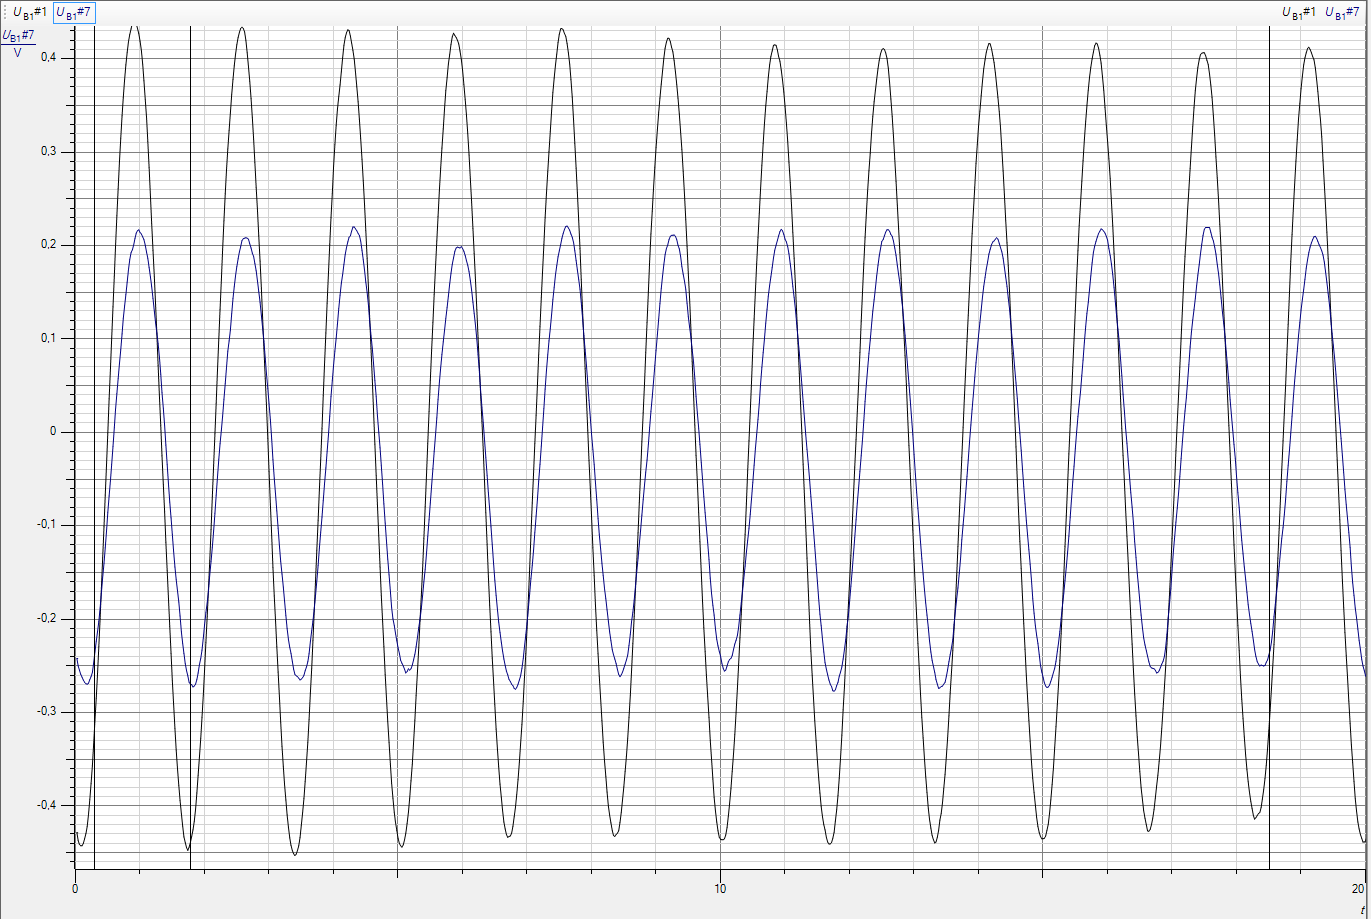
\includegraphics[width=1\textwidth]{phasenverschiebung_cassy_1.png}
	\caption{Analyse der Phasenverschiebung von Schwingung mit und ohne Pendelmasse im Labor mithilfe von Cassy-Lab, $t=[0s,20s]$}
	\label{fig:phasenverschiebung_cassy_1}
\end{figure}
\begin{figure}[H]
	\centering
	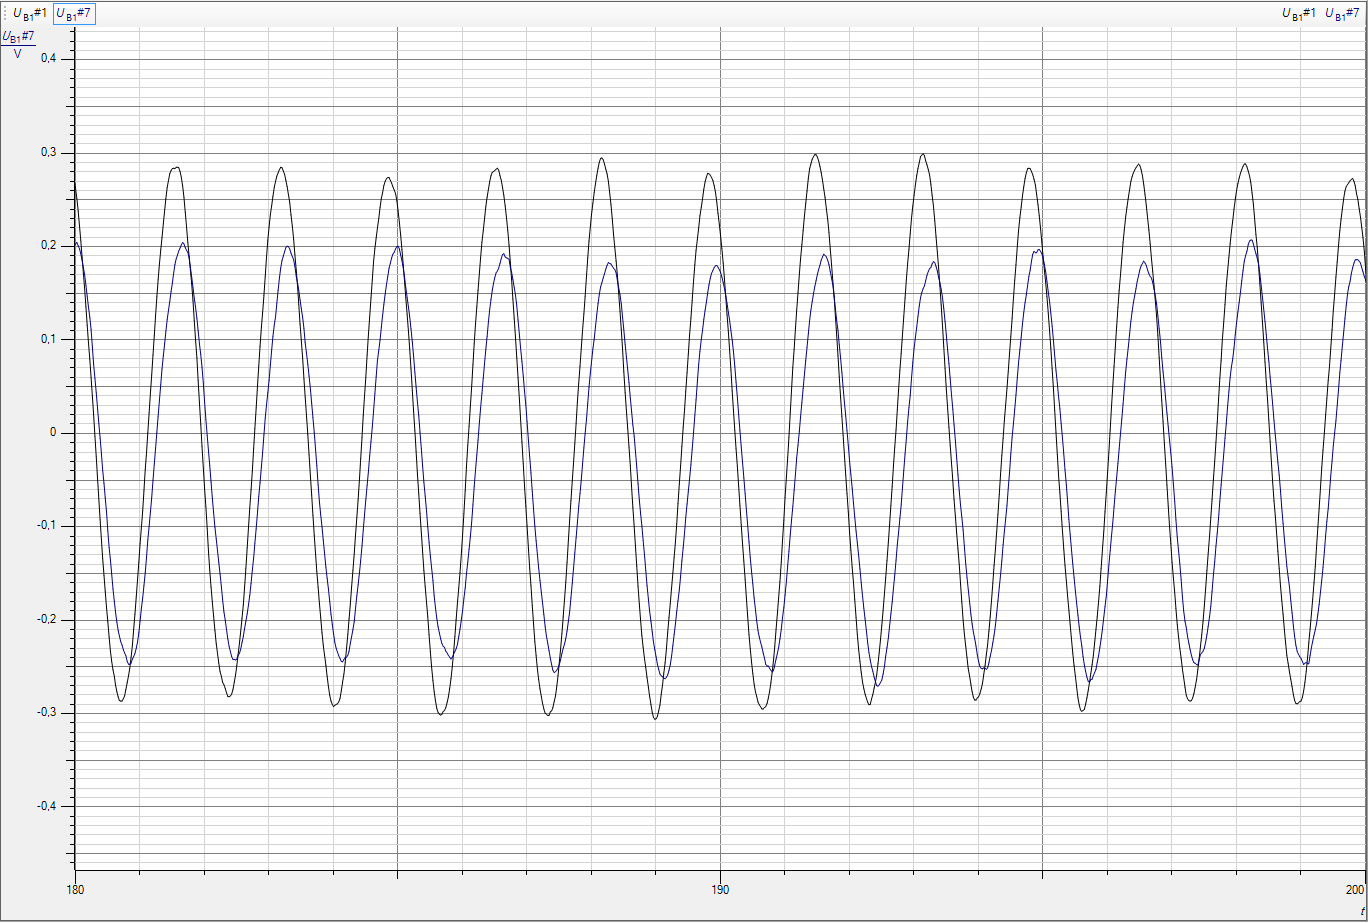
\includegraphics[width=1\textwidth]{phasenverschiebung_cassy_2.png}
	\caption{Analyse der Phasenverschiebung von Schwingung mit und ohne Pendelmasse im Labor mithilfe von Cassy-Lab, $t=[180s,200s]$}
	\label{fig:phasenverschiebung_cassy_2}
\end{figure}




\begin{aufgabe}{Rohdaten}
  Stellen Sie Ihre Rohdaten dar, tabellarisch für $l_p$ und $r_p$,
  grafisch für den Verlauf der Schwingung der Stange ohne Pendelkörper
  sowie der Pendelschwingung (für mindestens drei Messreihen).
\end{aufgabe}
Die Längen $l_p$ und $r_p$ haben wir nicht direkt bestimmt, sondern durch Teilmessungen erreicht um eine höhere Genauigkeit zu erzielen. Die Längen $a$ und $D$ wurden mit einem Messschieber bestimmt. Als statistischer Messfehler ergibt sich über die kleinste Skaleneinheit. Rein formal wäre $\sigma_{stat} = \frac{0.005cm}{\sqrt{12}}$. Eine solche Genauigkeit konnten wir jedoch nicht ablesen, weshalb für die folgenden Rechnungen einen statistischen Fehler von $\sigma_{stat} = 0.005cm$ annehmen. Einen systematischen Fehler konnten wir beim Messschieber ausschließen. Dazu haben wir den Messschieber maximal weit zusammengeschoben und eine Länge von exakt $0cm $ abgelesen. Die Länge $b$ haben wir mit einem Maßband vermessen. Hier ergibt sich der statistische Fehler wieder über die kleinste Skaleneinheit. Hier haben wir wieder auf den Faktor $\frac{1}{\sqrt{12}}$ verzichtet, da wir während das Pendel in der Aufhängung war, nicht eine solche Genauigkeit erreichen kommen. Hier verwenden wir also für die statistische Ungenauigkeit $\sigma_{stat} = 0.1cm$. Für die Messung wurde ein Maßband der Klasse II verwendet. Der Hersteller gibt hier einen systematischen Fehler von $\sigma_{syst}=0.3+0.2\cdot2 mm = 0.07cm$ an.\\
Mit diesem Angaben ergeben sich die Werte der Längenmessungen a, b und D samt Unsicherheit zu:\\
\begin{table}[hb]
	\centering
	\caption{Ergebnisse der Längenmessung für $a$}
	\label{tab:messwerte_a}
	\begin{tabular}{|c|c|c|c|}
		\hline
		Messung & $a\:[cm]$ & $\sigma_{stat}\: [cm] $ & $\sigma_{syst}\: [cm]$\\
		\hline
		$1$ & $3.00$ & $0.005$ & $0$\\
		\hline
		$2$ & $3.020$ & $0.005$ & $0$\\
		\hline
		$3$ & $3.010$ & $0.005$ & $0$\\
		\hline
	\end{tabular}
	\centering
	\caption{Ergebnisse der Längenmessung für $b$}
	\label{tab:messwerte_a}
	\begin{tabular}{|c|c|c|c|}
		\hline
		Messung & $b\:[cm]$ & $\sigma_{stat}\: [cm] $ & $\sigma_{syst}\: [cm]$\\
		\hline
		$1$ & $61.3$ & $0.1$ & $0.07$\\
		\hline
		$2$ & $61.3$ & $0.1$ & $0.07$\\
		\hline
		$3$ & $61.2$ & $0.1$ & $0.07$\\
		\hline
	\end{tabular}
	\centering
	\caption{Ergebnisse der Längenmessung für $D$}
	\label{tab:messwerte_a}
	\begin{tabular}{|c|c|c|c|}
		\hline
		Messung & $D\:[cm]$ & $\sigma_{stat}\: [cm] $ & $\sigma_{syst}\: [cm]$\\
		\hline
		$1$ & $7.980$ & $0.005$ & $0$\\
		\hline
		$2$ & $7.985$ & $0.005$ & $0$\\
		\hline
		$3$ & $7.995$ & $0.005$ & $0$\\
		\hline
	\end{tabular}
\end{table}\\
Die Abbildungen \ref{fig:Schwingung1_ohne} bis \ref{fig:Schwingung3_ohne} stellen die Rohdaten für die Pendelschwingung der Stange dar, Abbildungen \ref{fig:Schwingung1_mit} bis \ref{fig:Schwingung3_mit} für die Schwingung mit Pendelmasse. Die Rohdaten sollten formal in Form eines Scatterplots dargestellt werden. Um jedoch über den gesamten Messbereich eine gute Darstellung zu erreichen, haben wir lediglich die Verbindungslinien der einzelnen Messpunkte dargestellt. In Abbildung \ref{fig:zoomin_schwingung1_ohne} ist ein Zoom-In für die Schwingung der Stange (Messreihe 1) für die im Zeitintervall $\Delta t =10s$ dargestellt. Hier sind exemplarisch die tatsächlichen Messpunkte erkenntlich. 
\begin{figure}[H]
	\centering
	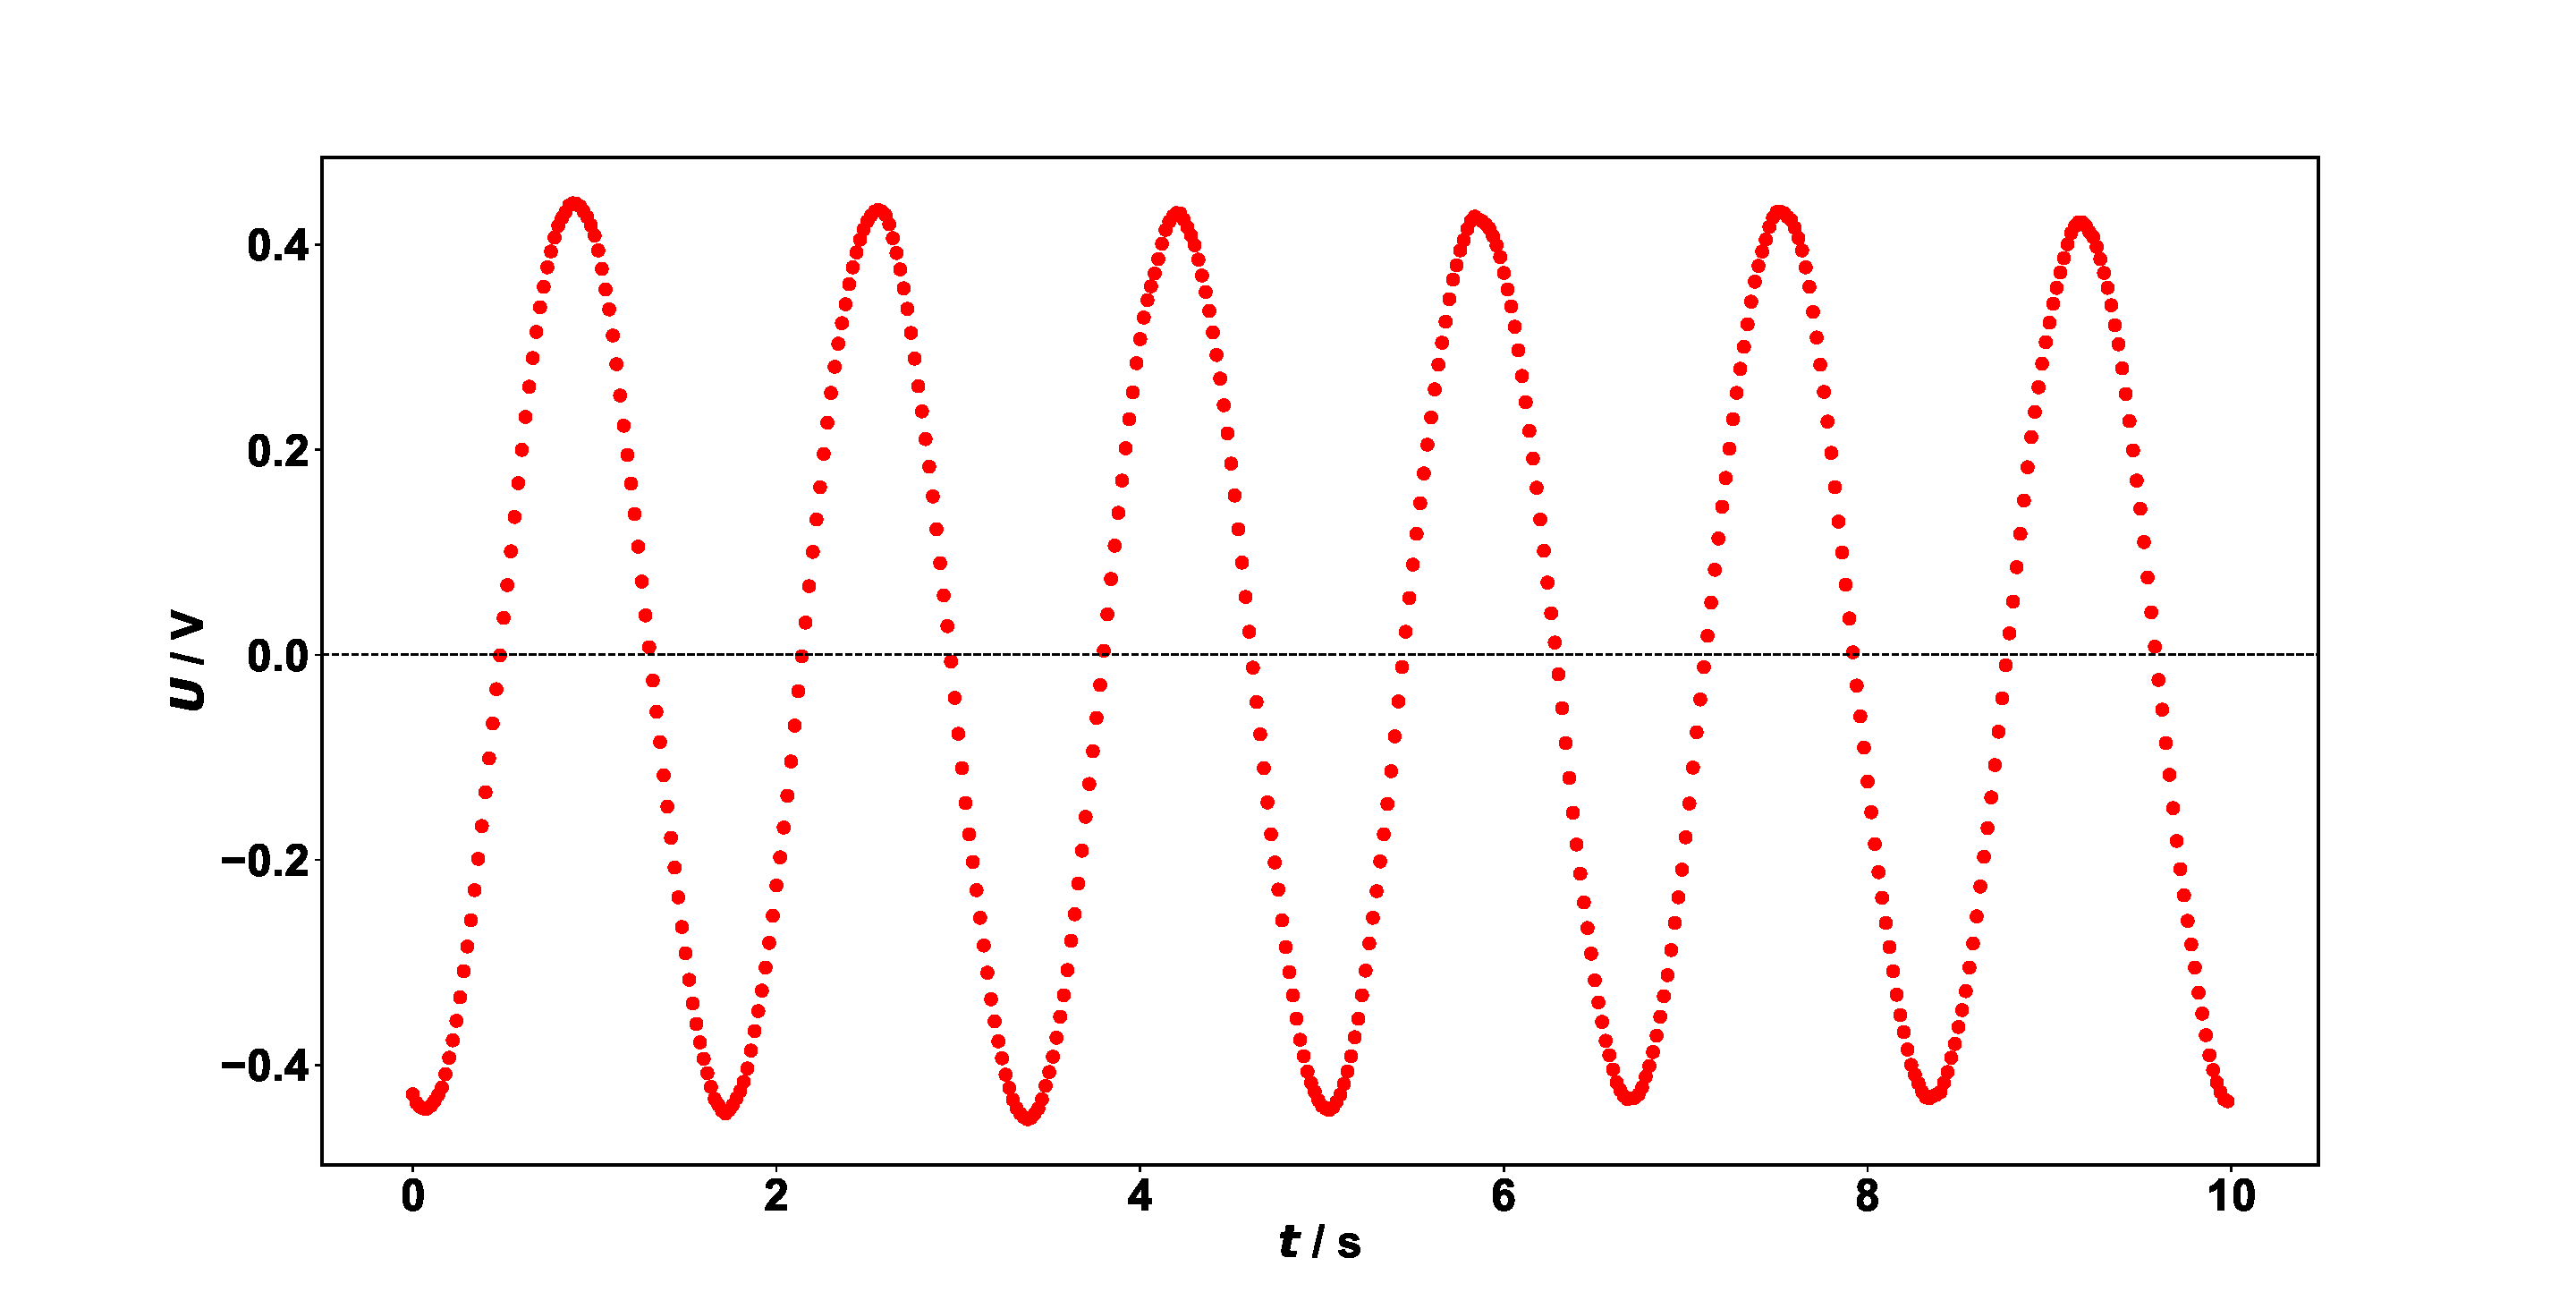
\includegraphics[width=1\textwidth]{zoomin_schwingung1_ohne.pdf}
	\caption{Zoom-In für die Schwingung ohne Pendelmasse, Messreihe 1}
	\label{fig:zoomin_schwingung1_ohne}
\end{figure} 



\begin{aufgabe}{Auswertung}
  Bestimmen Sie für alle Messreihen die Periodendauer und ihre
  Messunsicherheit, indem Sie eine geeignete lineare Regression
  durchführen. Demonstrieren Sie, dass Sie das Trägheitsmoment der
  Stange kompensiert haben. Tabellieren Sie die Zwischenergebnisse
  der relevanten Größen samt ihrer Messunsicherheiten. Berechnen
  Sie die Erdbeschleunigung. Führen Sie eine Fehlerrechnung zur
  Bestimmung der Messunsicherheit durch. Geben Sie bei Ihrer
  Fehlerrechnung die Größe der Einzelbeiträge an, die zu dem
  Gesamtfehler führen. Diskutieren Sie, welcher Fehler den
  Gesamtfehler dominiert. Vergleichen Sie Ihr Endergebnis mit dem
  relevanten Literaturwert.
\end{aufgabe}



%Anhang der Rohdaten%
\begin{figure}[H]
	\centering
	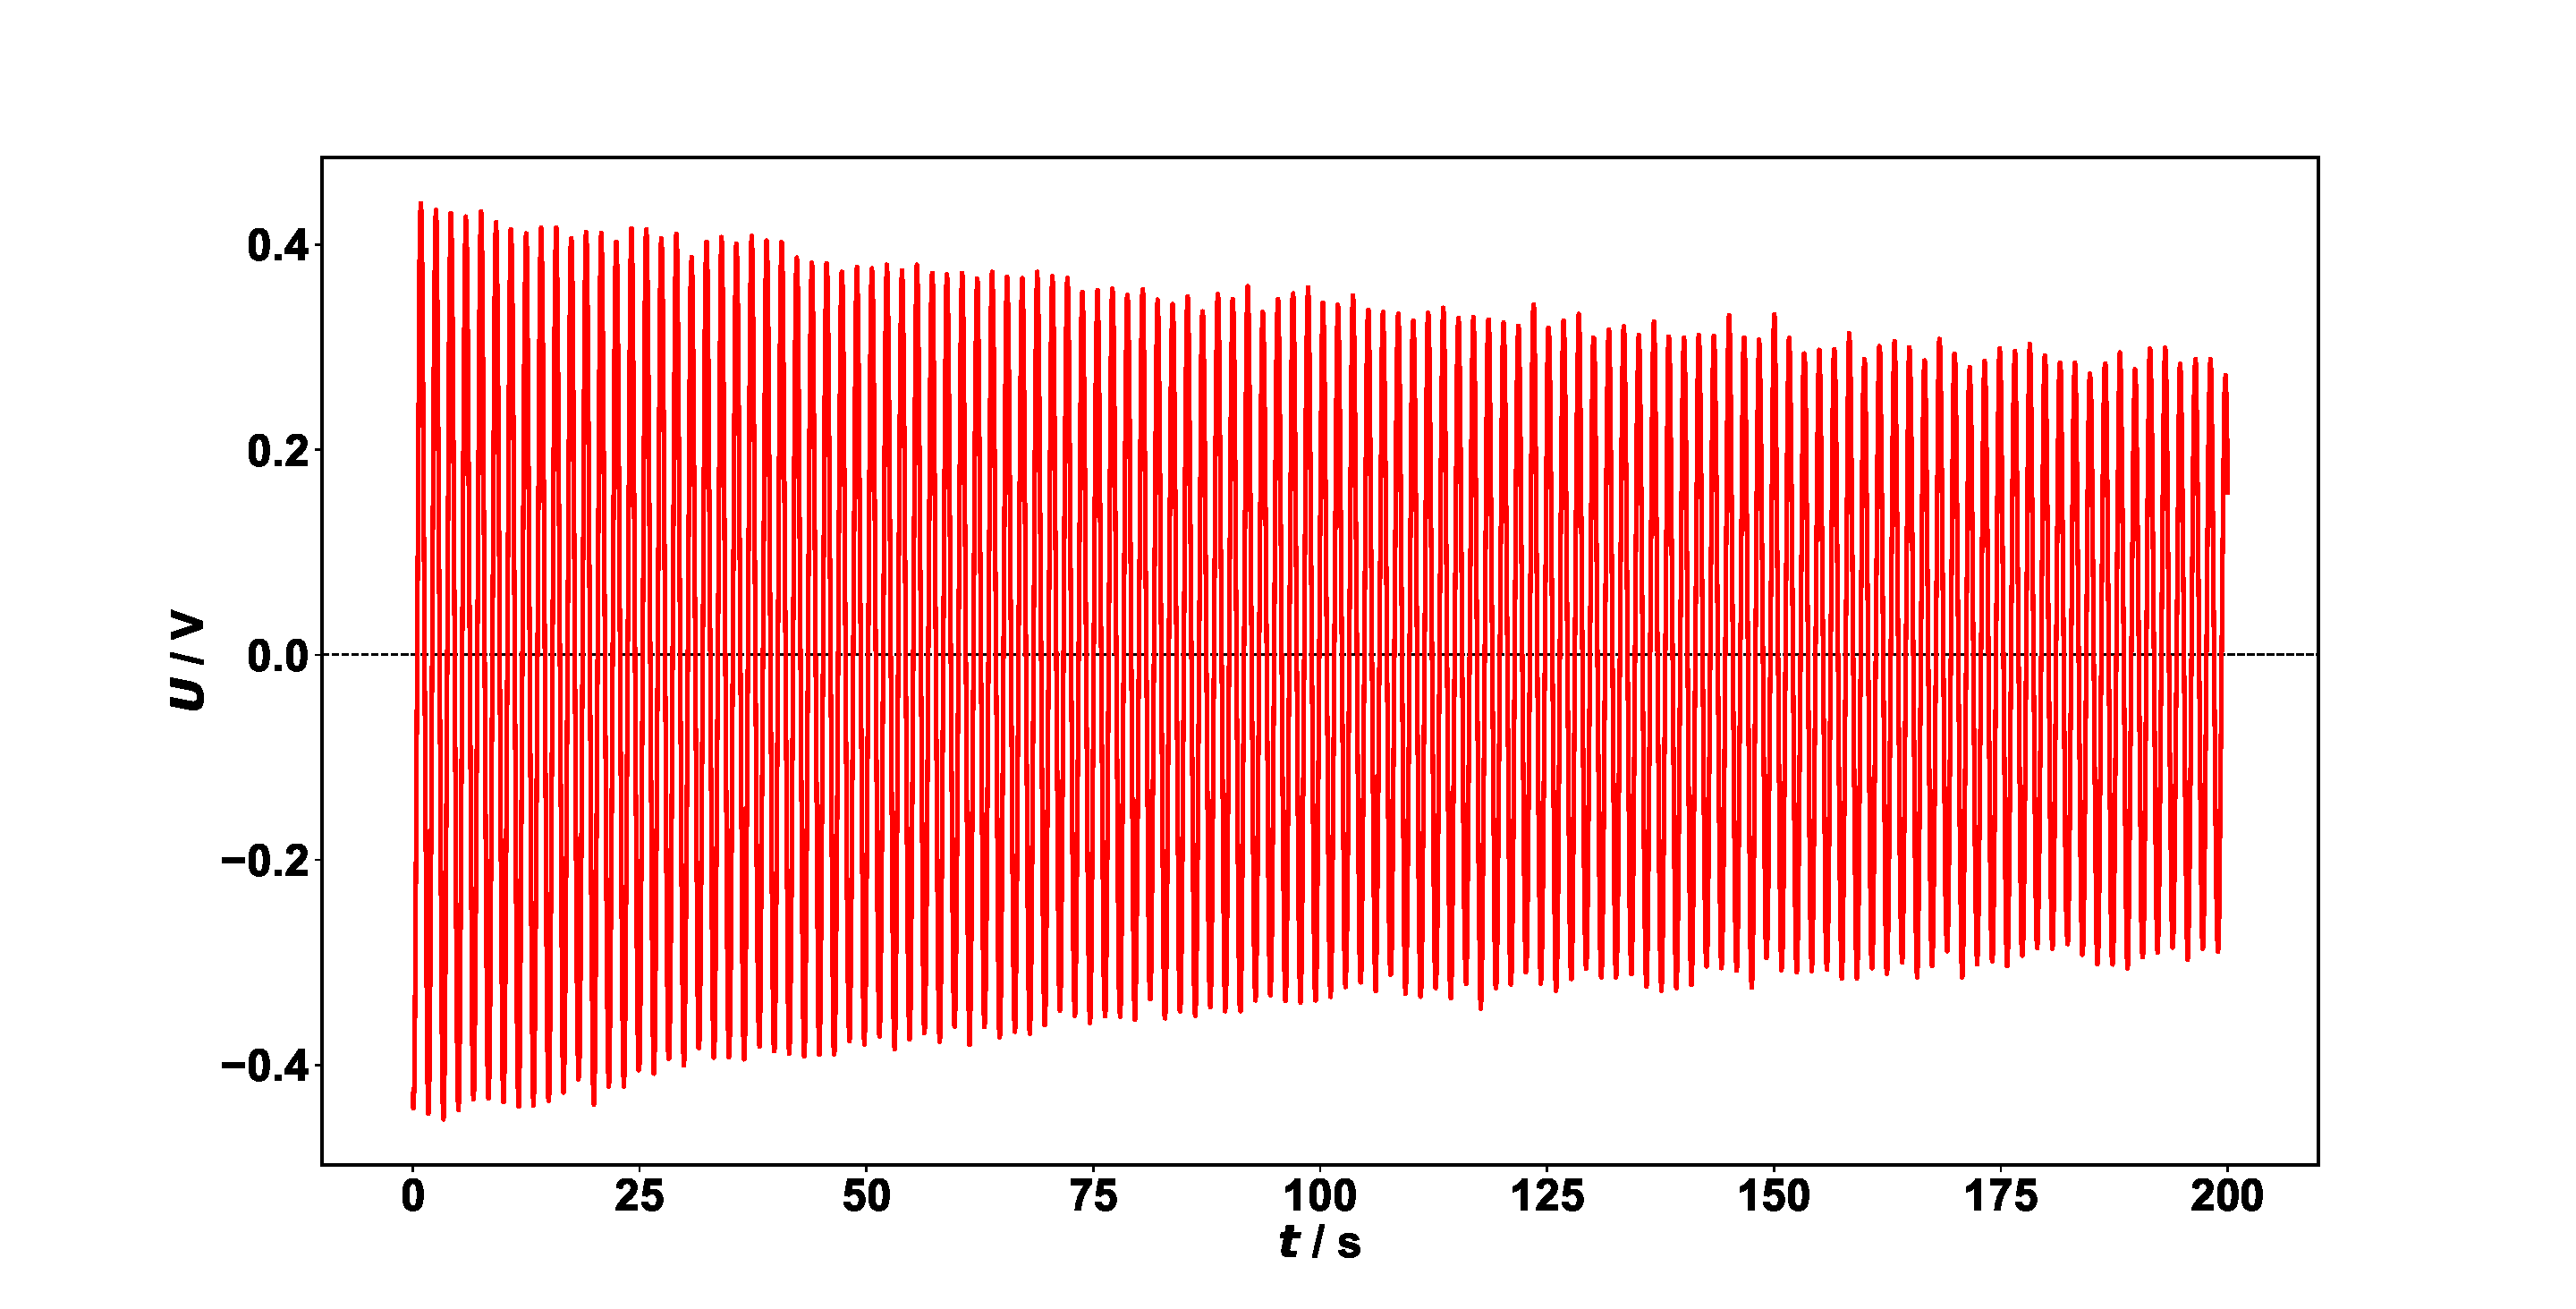
\includegraphics[width=1\textwidth]{Schwingung1_ohne.pdf}
	\caption{Schwingung ohne Pendelmasse, Messreihe 1}
	\label{fig:Schwingung1_ohne}
\end{figure}
\begin{figure}[H]
	\centering
	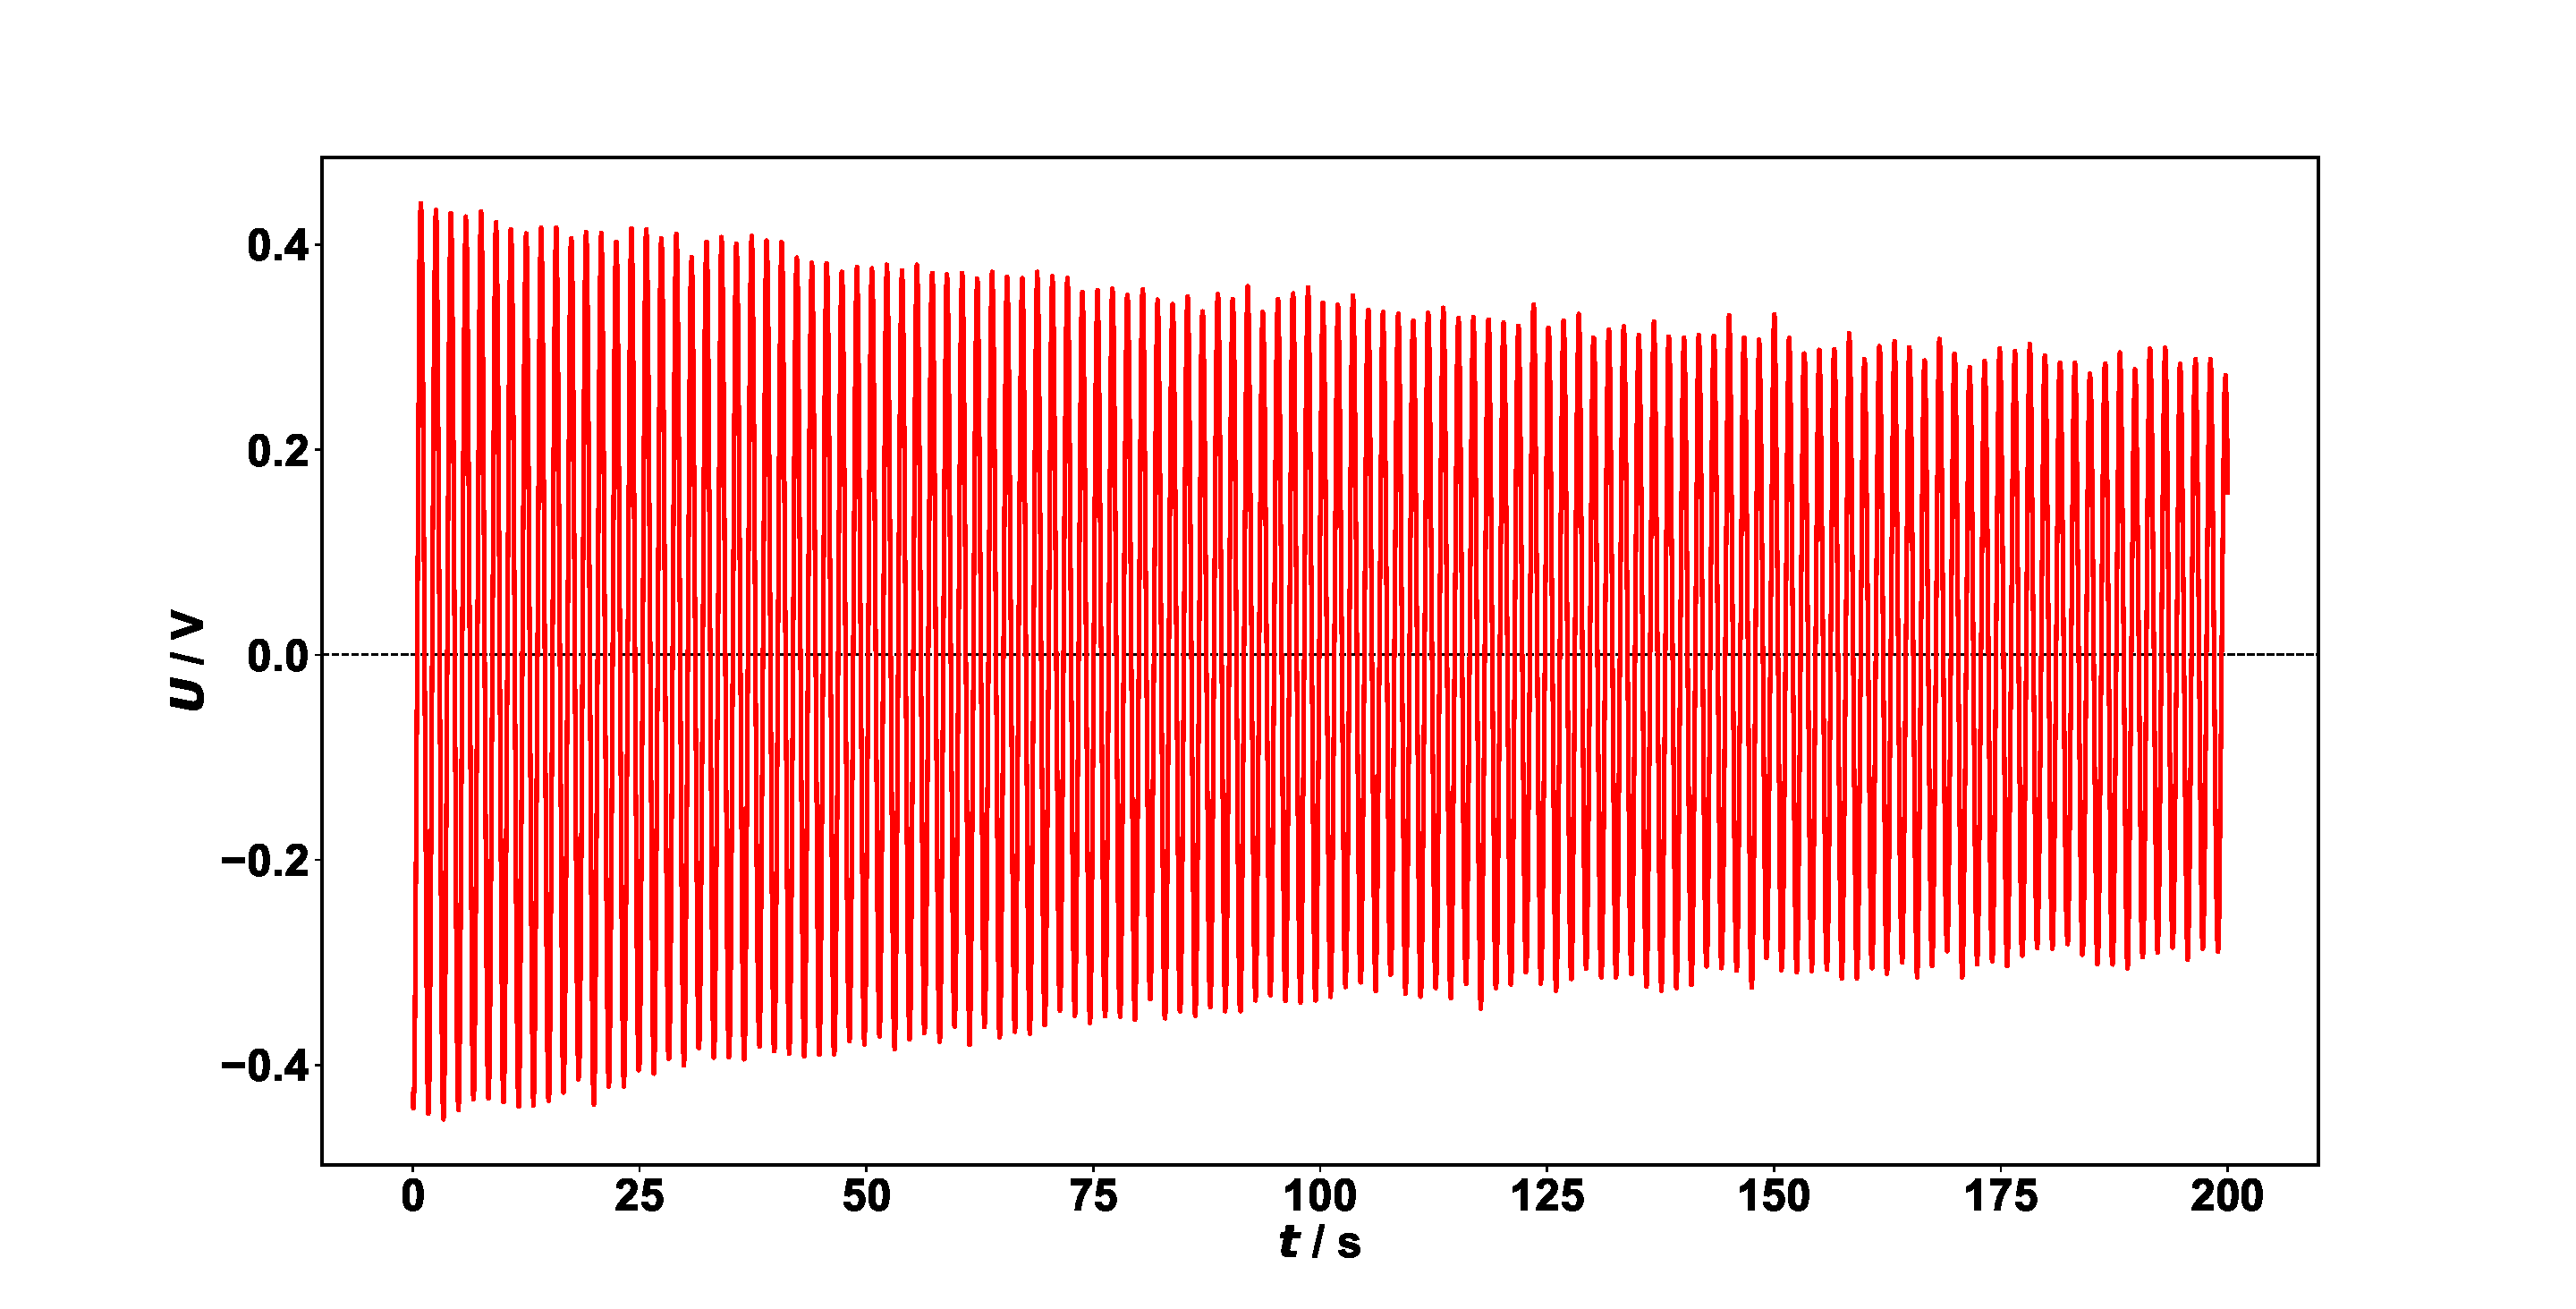
\includegraphics[width=1\textwidth]{Schwingung2_ohne.pdf}
	\caption{Schwingung ohne Pendelmasse, Messreihe 2}
	\label{fig:Schwingung2_ohne}
\end{figure}
\begin{figure}[H]
	\centering
	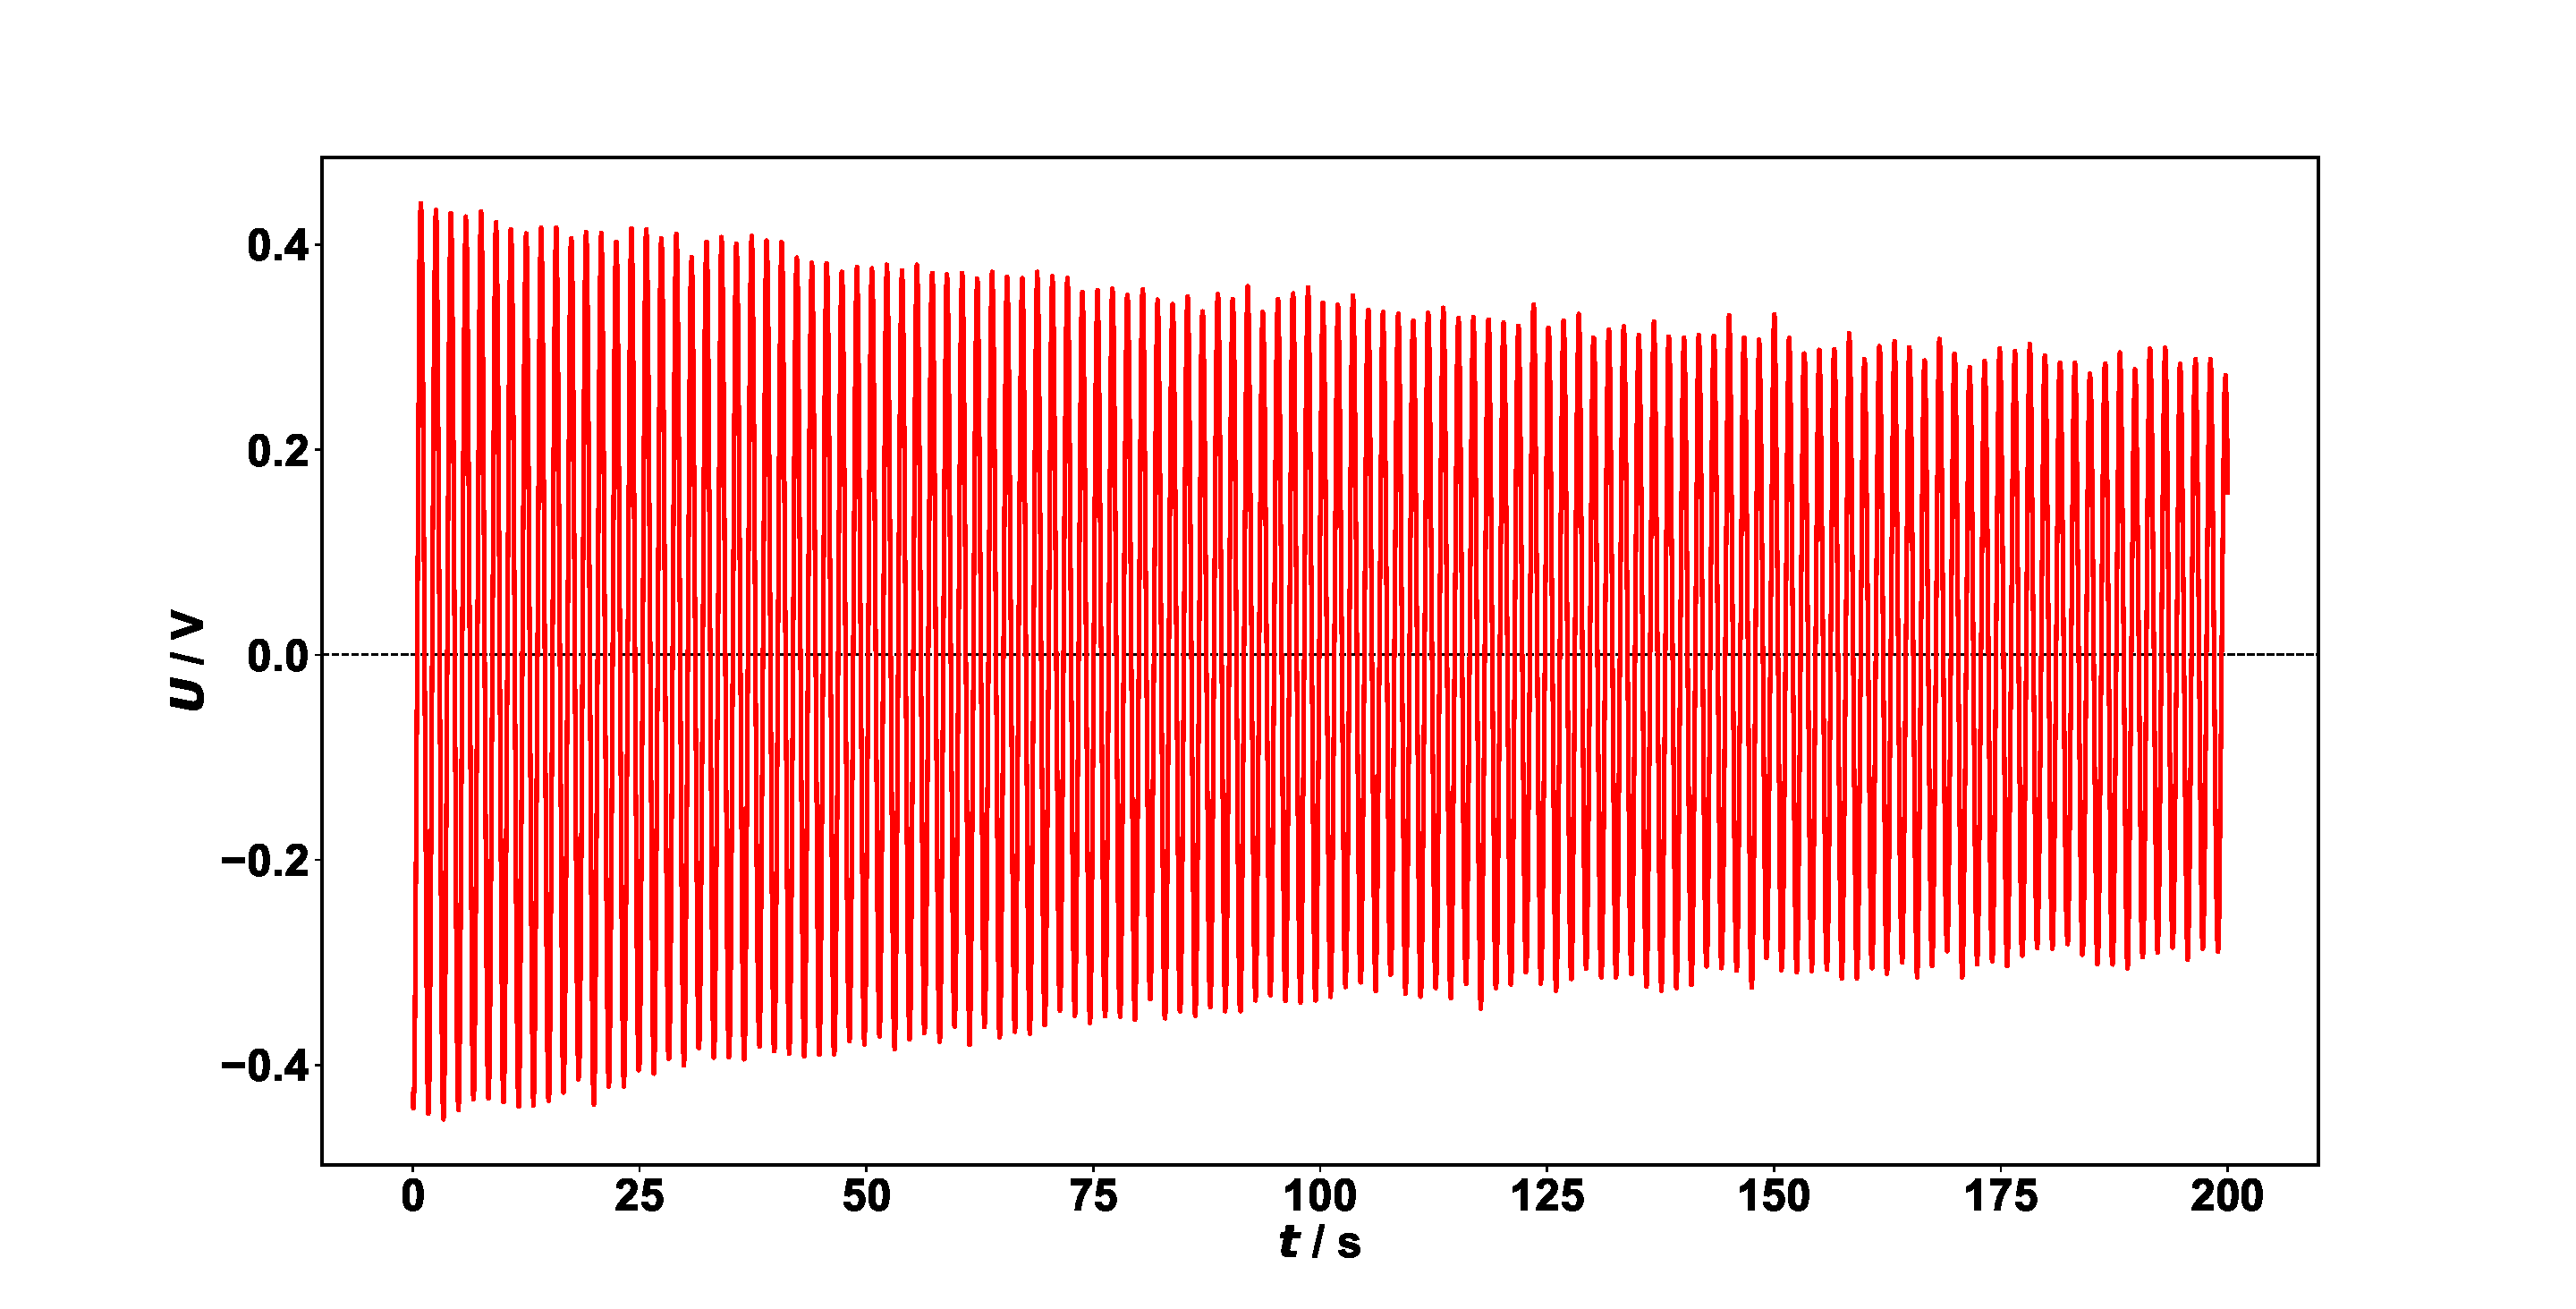
\includegraphics[width=1\textwidth]{Schwingung3_ohne.pdf}
	\caption{Schwingung ohne Pendelmasse, Messreihe 3}
	\label{fig:Schwingung3_ohne}
\end{figure}
\begin{figure}[H]
	\centering
	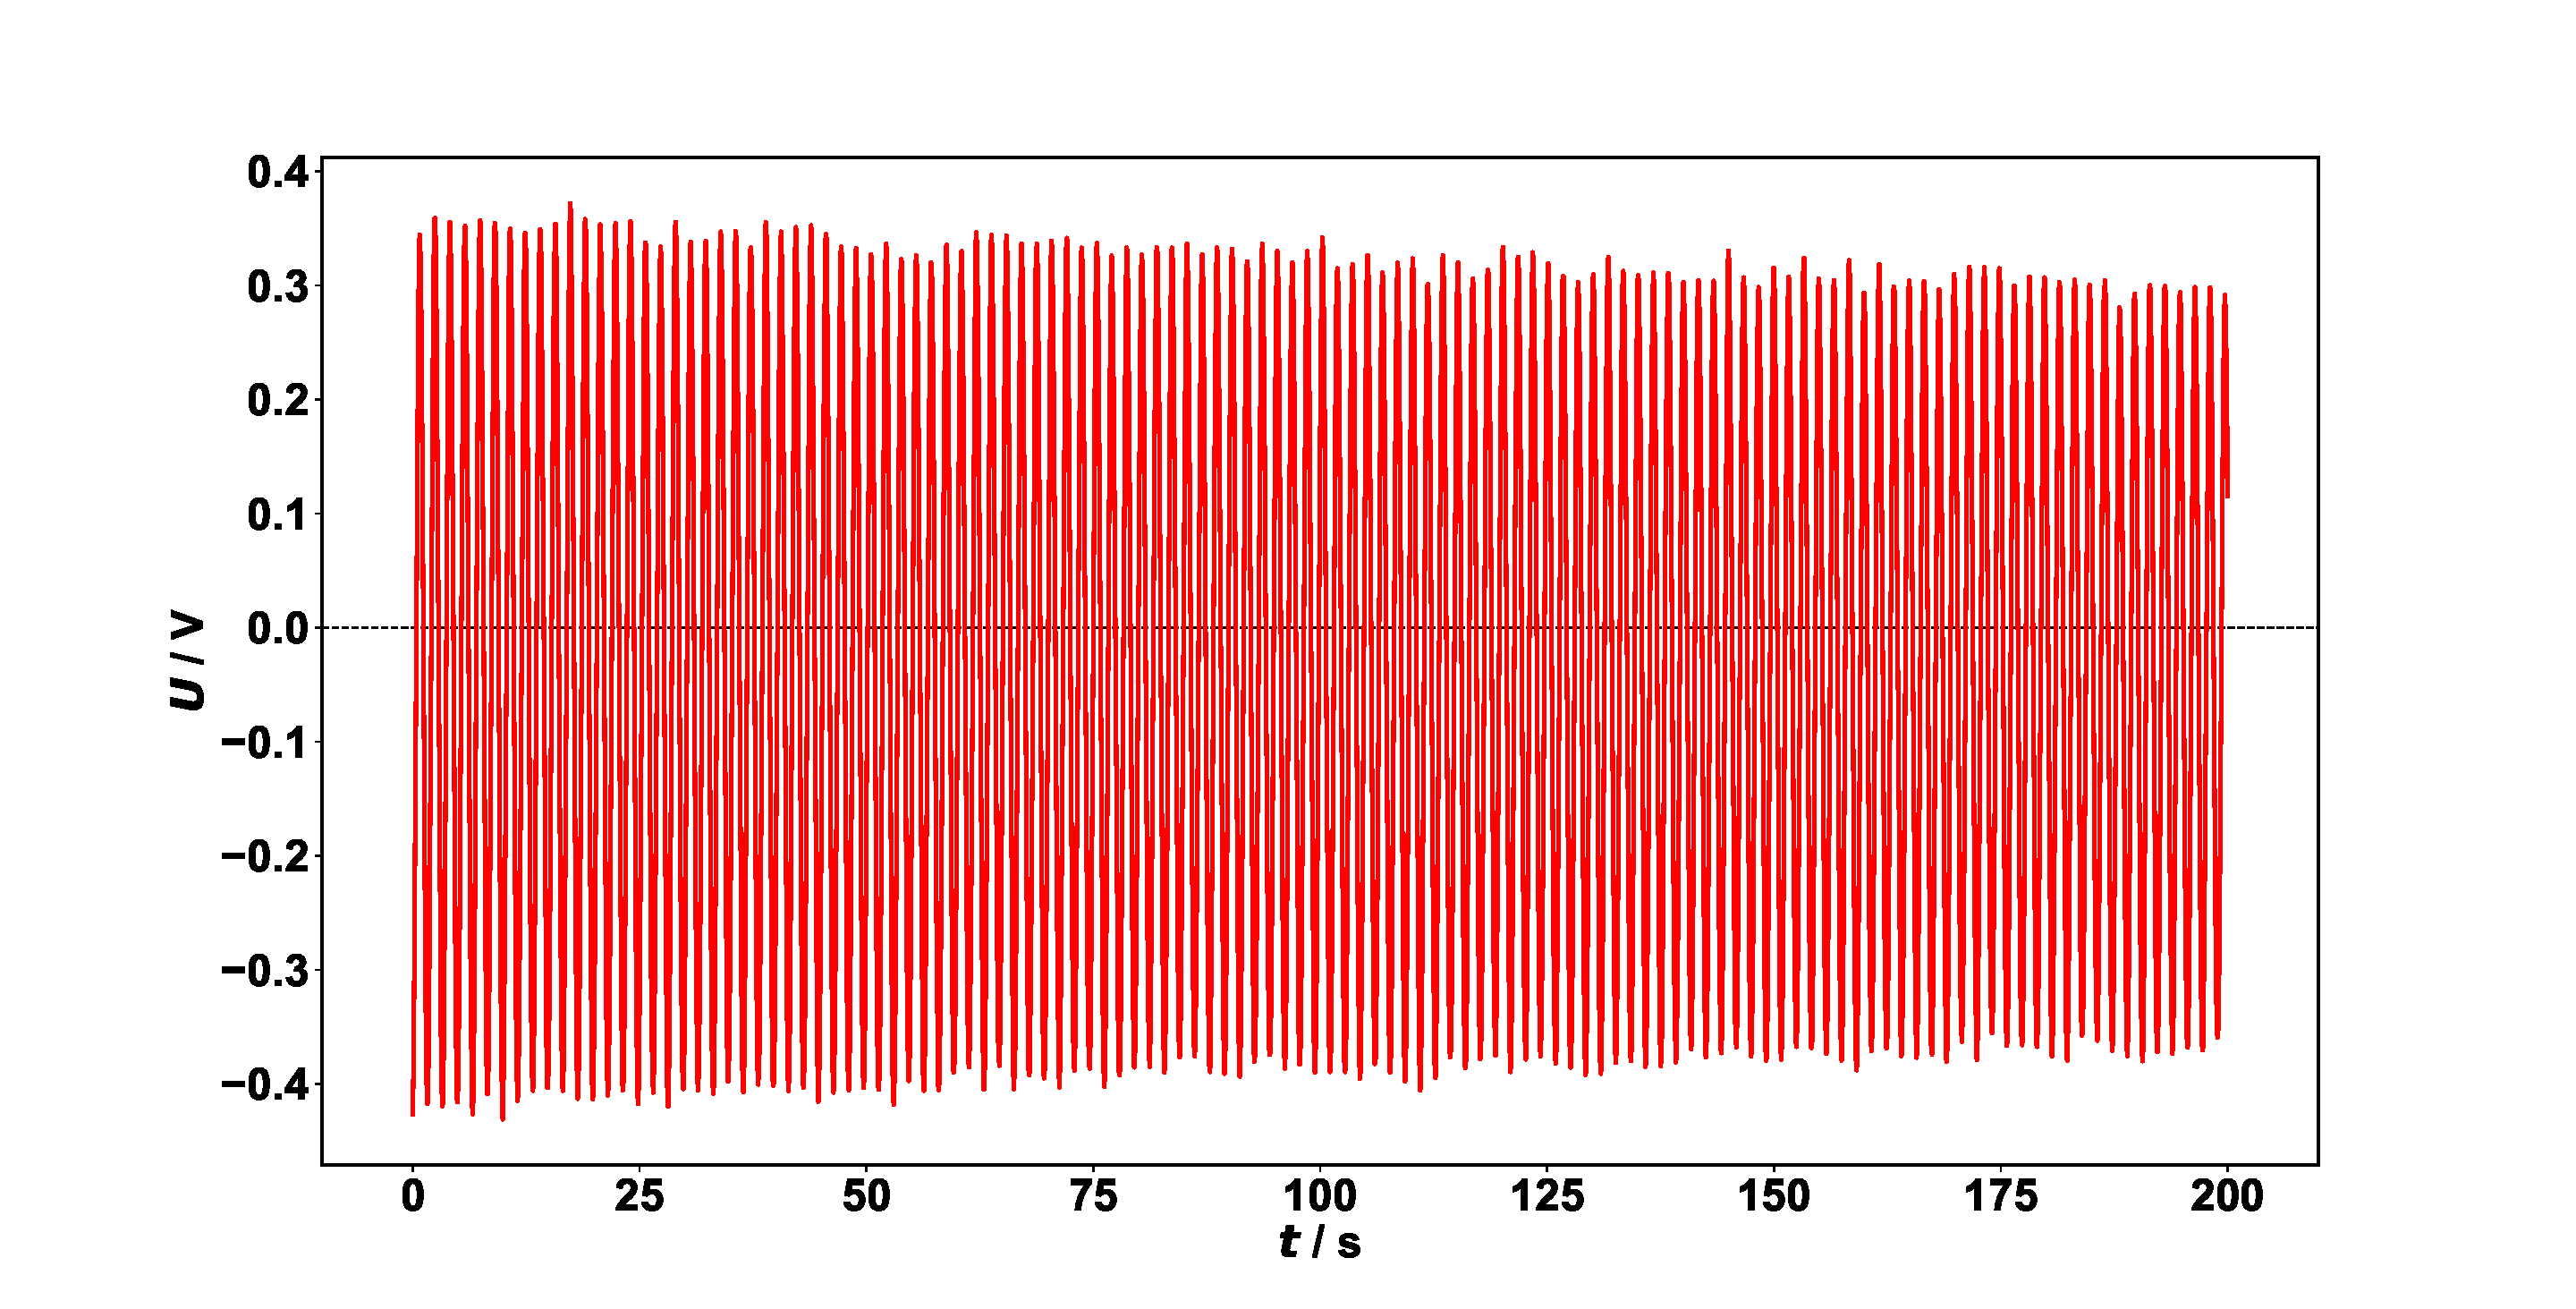
\includegraphics[width=1\textwidth]{Schwingung1_mit.pdf}
	\caption{Schwingung mit Pendelmasse, Messreihe 1}
	\label{fig:Schwingung1_mit}
\end{figure}
\begin{figure}[H]
	\centering
	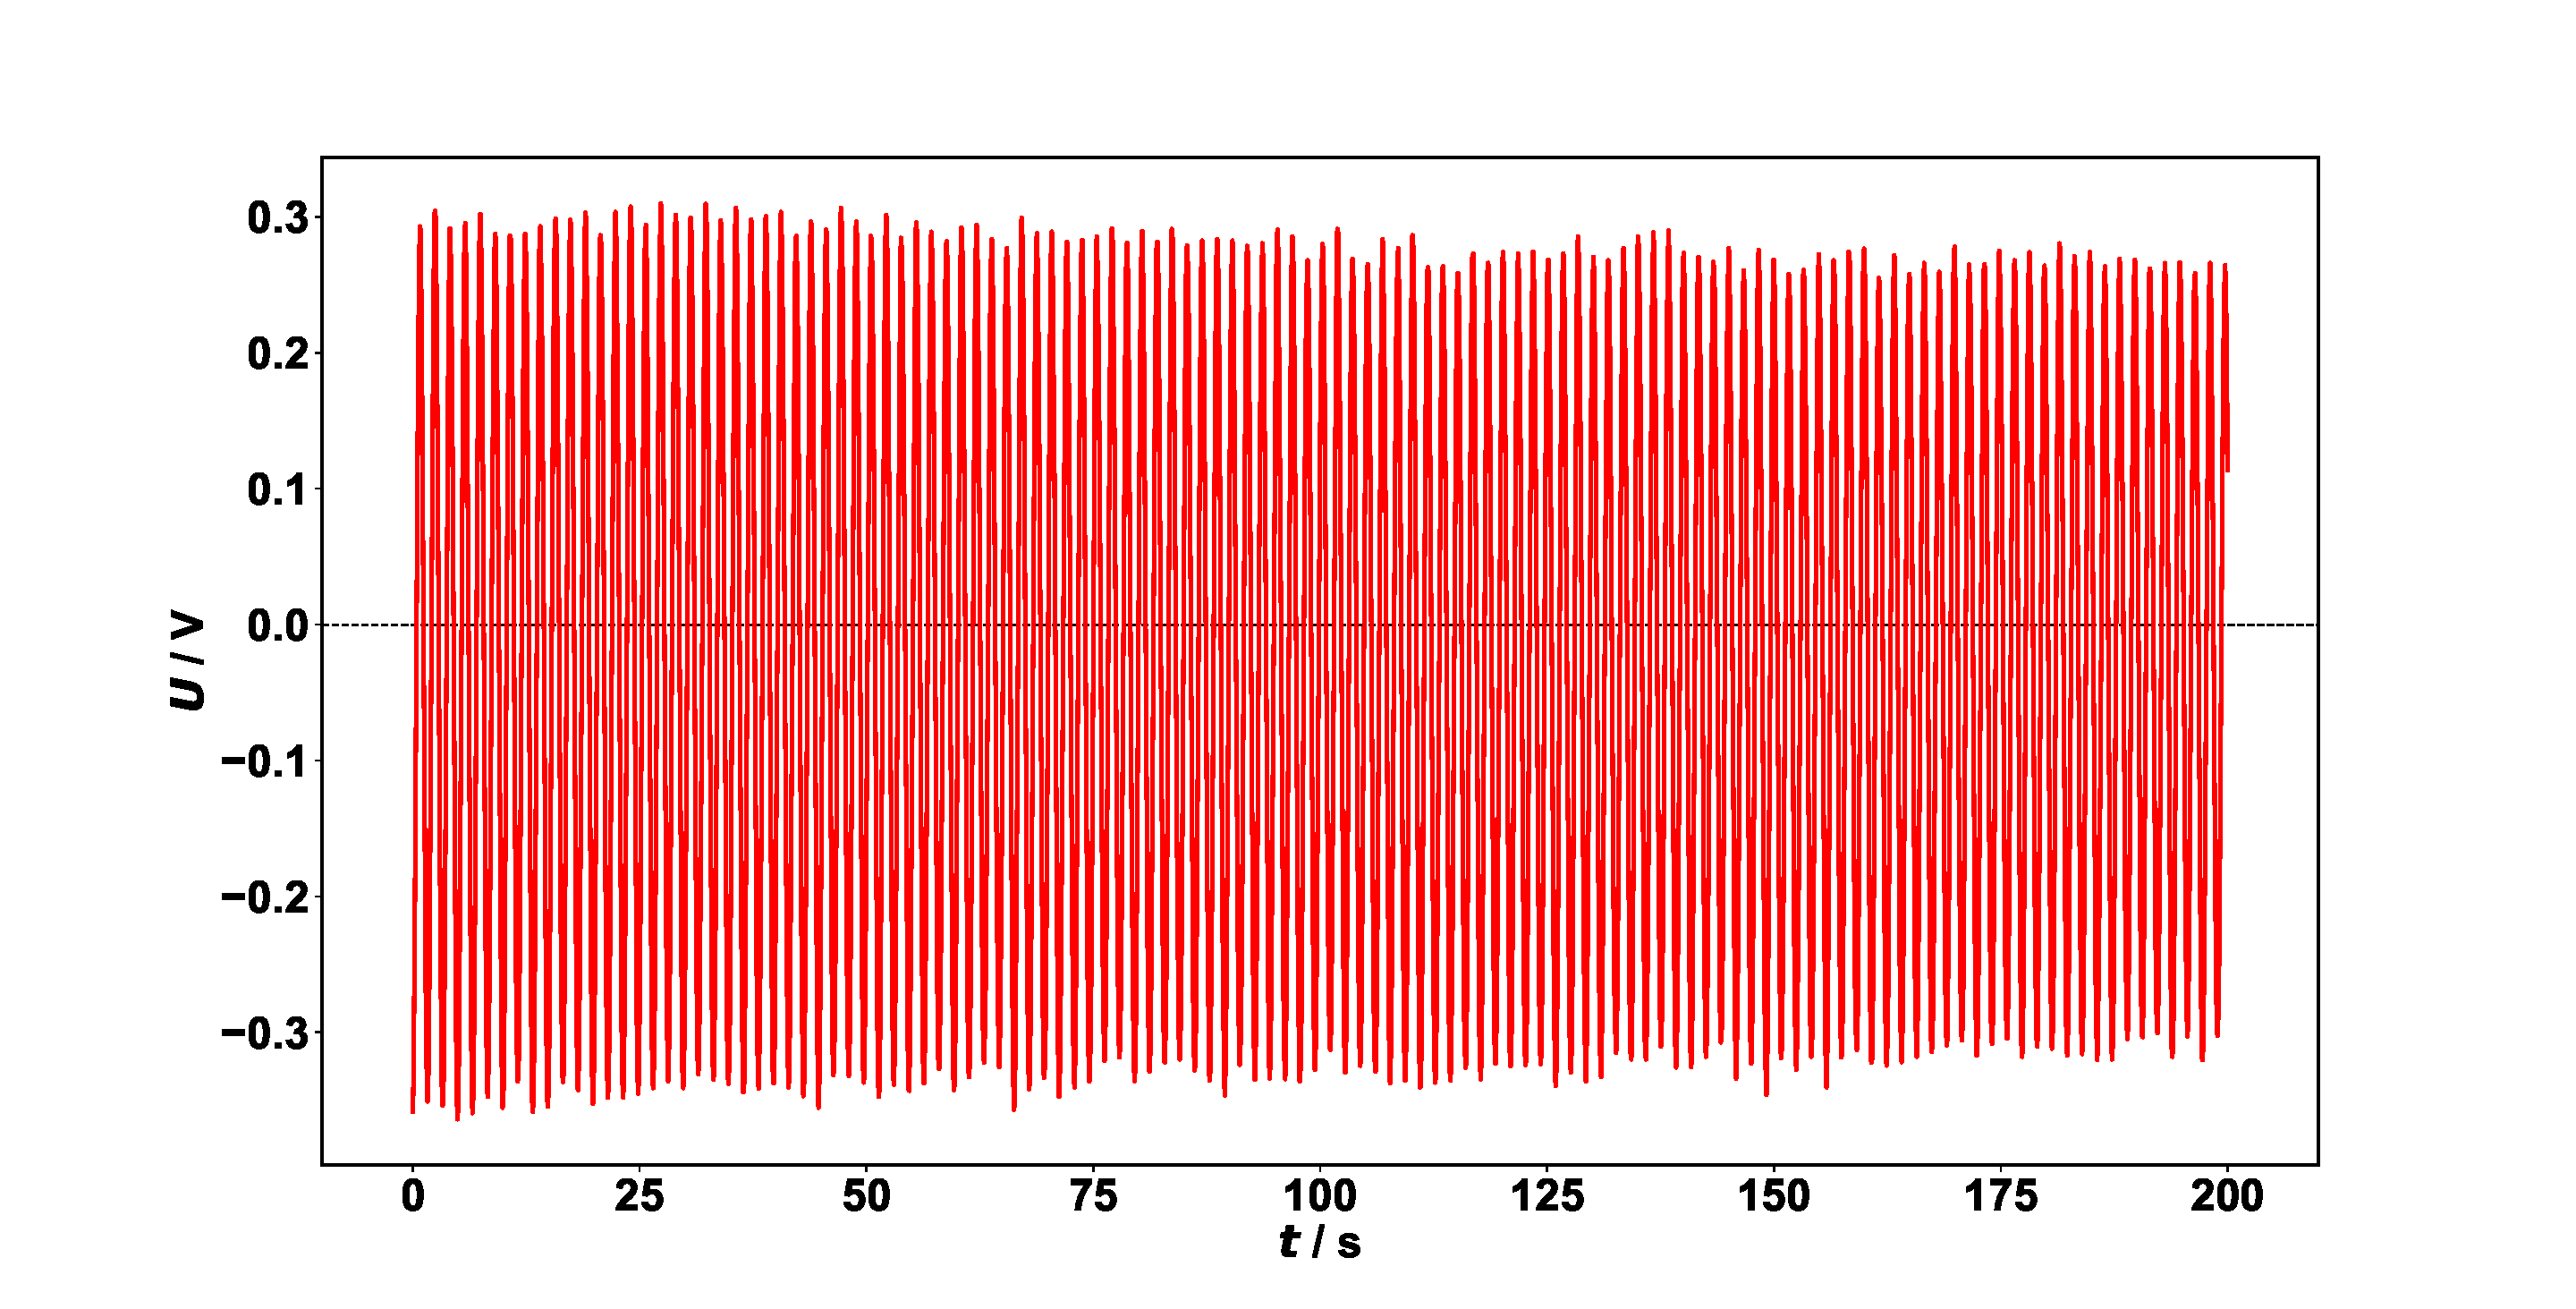
\includegraphics[width=1\textwidth]{Schwingung2_mit.pdf}
	\caption{Schwingung mit Pendelmasse, Messreihe 2}
	\label{fig:Schwingung2_mit}
\end{figure}
\begin{figure}[H]
	\centering
	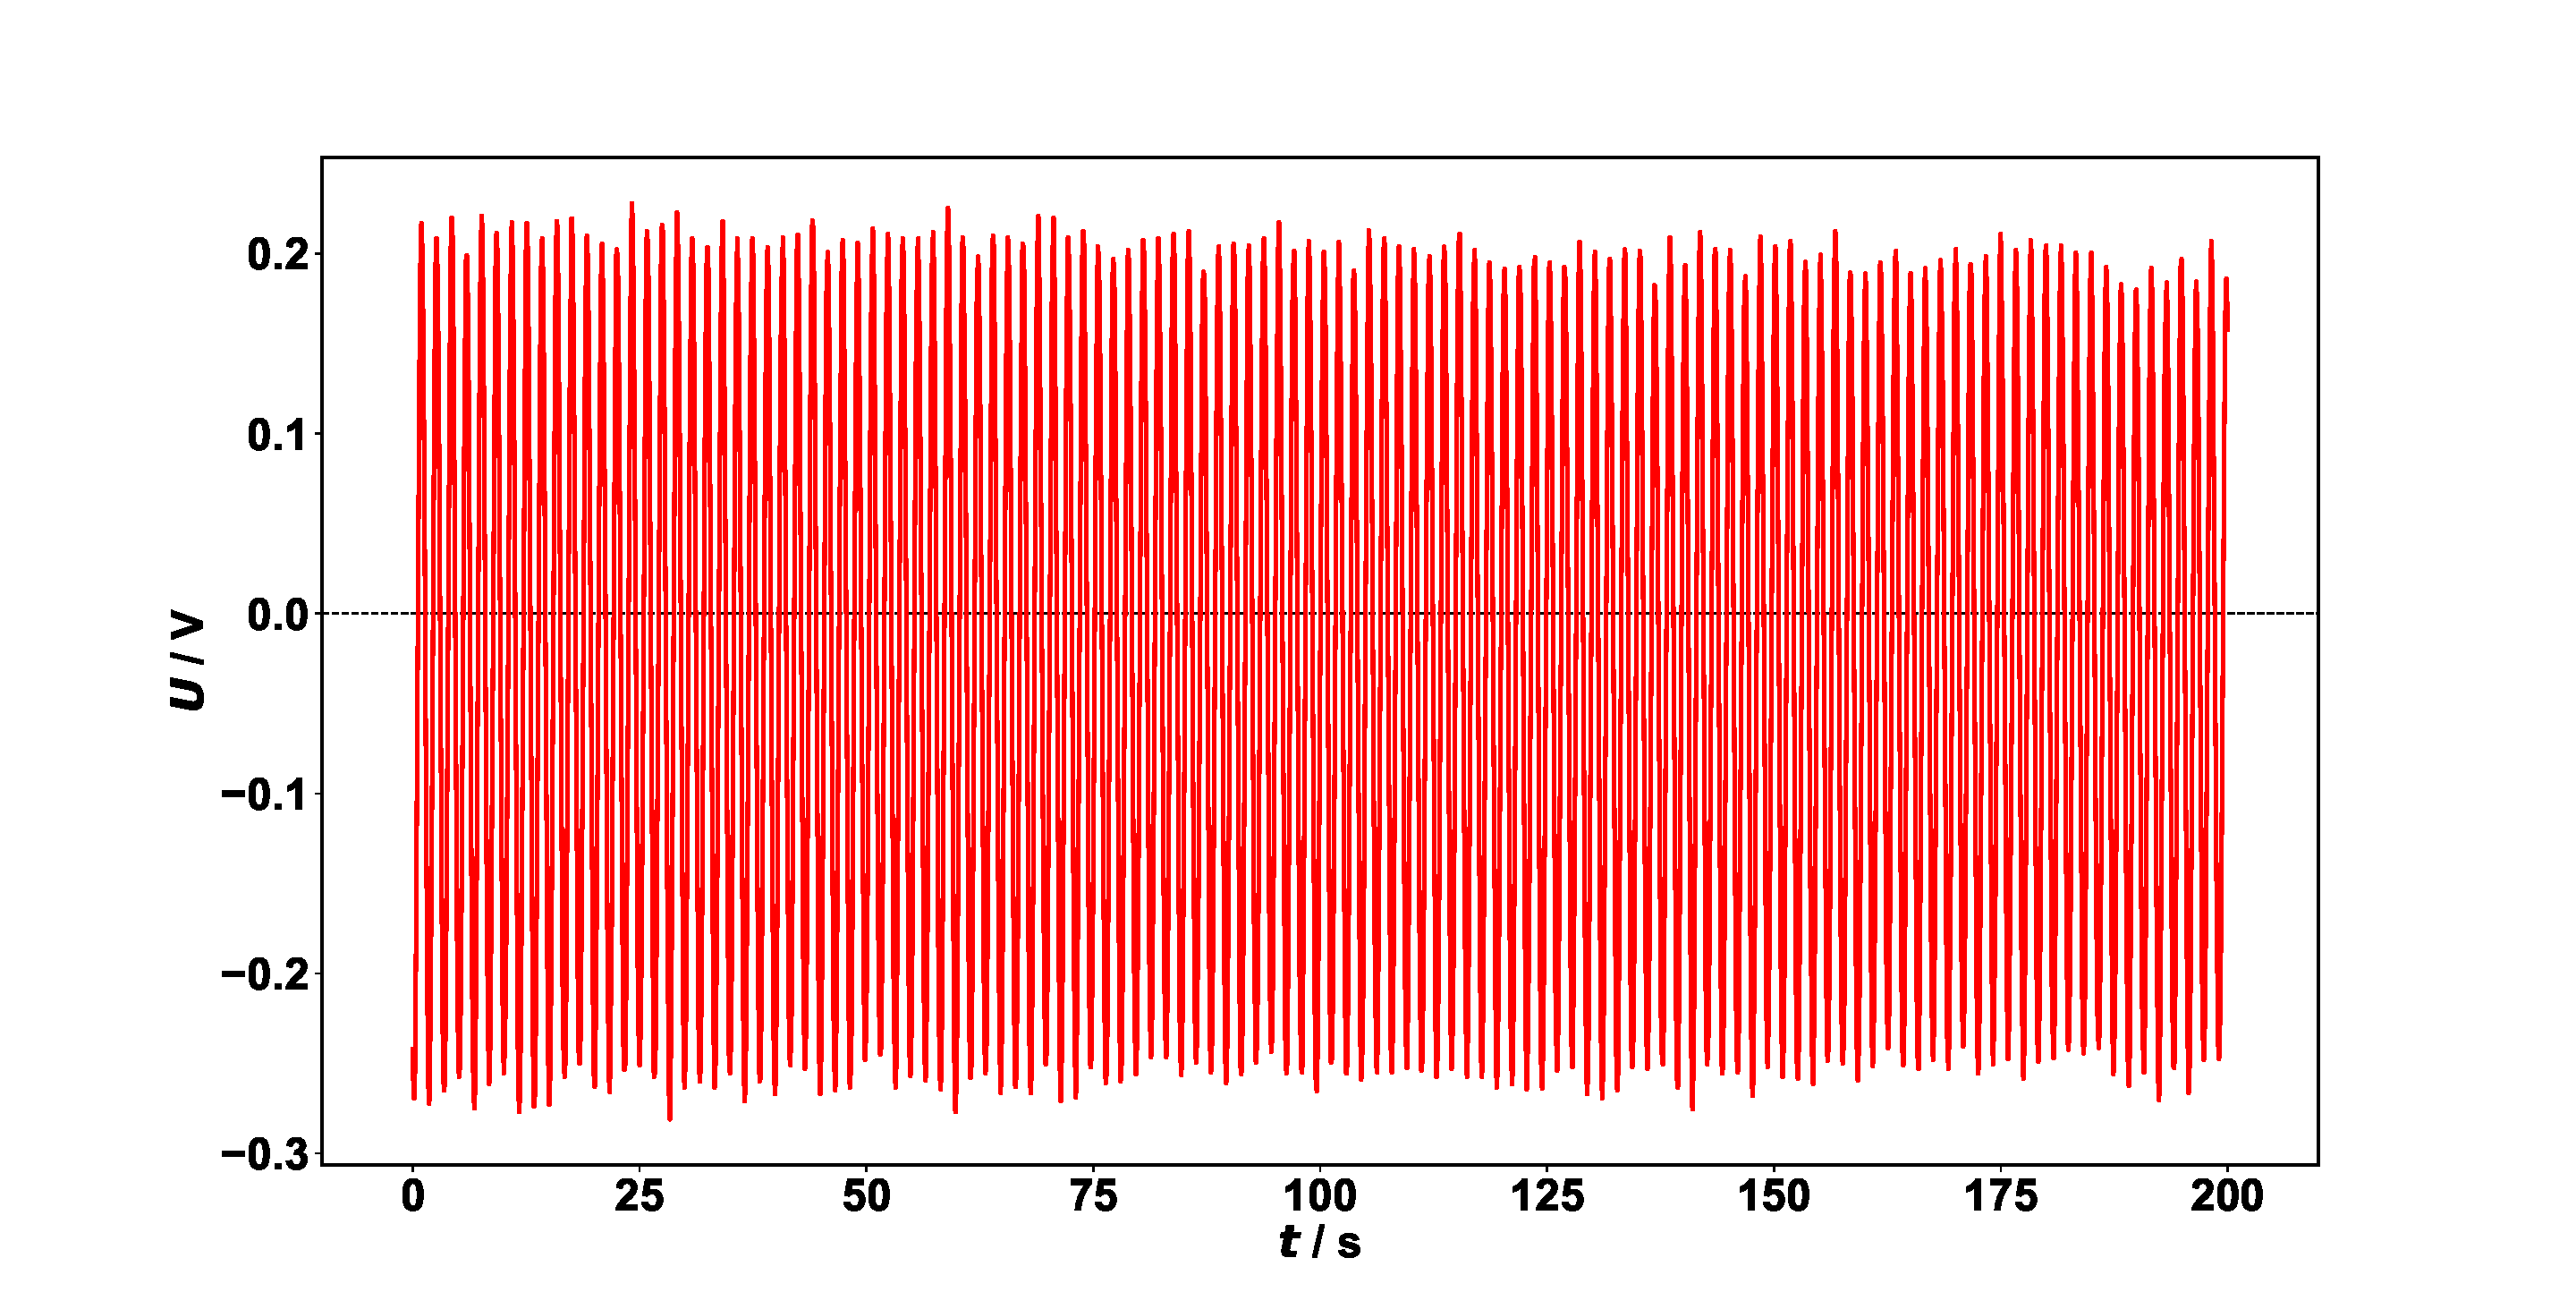
\includegraphics[width=1\textwidth]{Schwingung3_mit.pdf}
	\caption{Schwingung mit Pendelmasse, Messreihe 3}
	\label{fig:Schwingung3_mit}
\end{figure}

